
%\newpage
\section{Selbsttest Funktion}
\label{sec:selftest}
Beginnend mit Version 0.9k habe ich eine Selbsttest-Funktion eingebaut.
Die Benutzung ist sehr einfach.
Wenn Sie Pr\"ufspitzen mit Klemmen verwenden, klemmen Sie alle Klemmen auf ein unisoliertes St\"uck Draht und dr\"ucken Sie
den Start Taster.
Das Programm bemerkt die kurzgeschlossenen Klemmen und startet den Selbsttest.
Nach Beenden des Selbsttestes wird der Tester mit normaler Messung fortfahren.
Wenn kein Bauteil angeschlossen ist, wird der TransistorTester mit der
Meldung ,,kein,unbek. oder defektes Bauteil'' enden.
Die ungl\"uckliche Seite der Selbsttest-Funktion ist, da"s der 8k flash Speicher fast verbraucht ist.
Die L\"ange der ATmega8 Version ist ungef\"ahr 8000 Bytes.
Man kann die Selbsttest-Funktion zusammen mit allen anderen Optionen nur f\"ur einen ATmega168
oder ATmega328 w\"ahlen.
F\"ur einen ATmega8 mu"s man wegen des begrenzten flash Speichers wenigstens die Option AUTOSCALE\_ADC weglassen.
Die einzelnen Schritte der Selbsttestfunktion werden immer in Zeile~1 des LCD Displays mit dem Buchstaben T
gefolgt von der Schritt-Nummer dargestellt.
Jeder Schritt wird achtmal wiederholt, bevor das Programm zum n\"achsten Schritt geht.
Aber wenn man den Start Taster gedr\"uckt h\"alt, wenn ein Durchlauf beendet wird, wird dieser Test nicht
mehr wiederholt.
Wenn man den Taster w\"ahrend dem gesamten Selbsttest gedr\"uckt h\"alt, wird jeder Schritt nur einmal ausgef\"uhrt.

Ohne die AUTO\_CAL Option werden in jedem Schritt nur Me"sergebnisse dargestellt, es wird keine Fehleranalyse durchgef\"uhrt.
Man  mu"s die Ergebnisse selbst interpretieren.
An dieser Stelle m\"ochte ich noch einen wichtigen Hinweis geben. F\"uhren Sie niemals Messungen mit
eingestecktem ISP-Stecker durch!
Die ISP-Schnittstelle st"ort die Messungen.

\vspace{1cm}
Hier ist die Liste der derzeit eingebauten Tests:
\vspace{1cm}
\begin{enumerate}
\item {\bf Messung der 1,3V (oder 1,1V) Referenz Spannung (band gap Reference).} In Zeile~1 wird der Text ,,Ref='' und die
gemessene Spannung in mV angezeigt.
F\"ur den ATmega8 sollte die gemessene Spannung nahe bei 1,3V liegen, f\"ur die anderen Prozessoren liegt
die Referenzspannung normal um die 1,1V.
Die zweite Zeile zeigt den resultierenden Faktor f\"ur die Kapazit\"ats-Messung mit dem \(470k\Omega\) Widerstand.
\item {\bf Vergleich der \(680\Omega\) Widerst\"ande.} 
In Zeile~1 wird der kryptische Text  ,,+RL- 12 13 23'' angezeigt. Das bedeutet das folgende:
Das RL ist eine Kurzform f\"ur Resistor Low, was die \(680\Omega\) Widerst\"ande meint. Die ,,12'' steht f\"ur: 
Widerstand am Pin~1 ist verbunden mit VCC (+) und Widerstand am Pin~2 ist verbunden mit GND (-). 
Das Ergebnis dieser Messung steht in Zeile~2 an erster Stelle als Differenz zum theoretischen Wert.
 In Zeile~1 folgt nun ,,13'', was bedeutet, da"s der Widerstand von Pin~1 wieder nach VCC verbunden ist,
aber da"s jetzt der \(680\Omega\) Widerstand von Pin~3  mit GND verbunden ist.
Das Ergebnis steht in Zeile 2 an der mittleren Stelle als Differenz zum theoretischen Wert.

Die letzte Messung dieses Tests ,,23'' bedeutet, da"s nun der Widerstand von Pin~2 mit VCC verbunden ist und
der Widerstand von Pin~3 mit GND verbunden ist.
Das Ergebnis steht in der zweiten LCD-Zeile an letzter Stelle als Differenz zum theoretischen Wert.
Ich m\"ochte daran erinnern, da"s die Aufl\"osung des ADC etwa 4,88mV betr\"agt!
Die Me"ssituation wird auch in Abbildung~\ref{fig:test2} dargestellt.
Der theoretische Wert ergibt sich im Hinblick auf die internen Port-Widerst\"ande wie folgt:
\(\frac{5001 \cdot  (19+680)}{ (19+680+680+22)} = 2493\) .

\begin{figure}[H]
\centering

\includegraphics[width=17cm]{../FIG/Test2.eps}
\caption{Vergleich der \(680\Omega\) Widerst\"ande }
\label{fig:test2}
\end{figure}

\item {\bf Vergleich der \(470k\Omega\) Widerst\"ande.}
Jetzt zeigt das Display in Zeile 1 ,,+RH- 12 13 23''. Das gleiche Verfahren wie in Schritt wird wiederholt mit den
 \(470k\Omega\) Widerst\"anden (Symbol RH).
Die Ergebnisse werden als Differenz zu  \(\frac{VCC \cdot (19 + 470000]}{ (19 + 470000 + 470000 + 22)} \) f\"ur alle Kombinationen dargestellt.
\item In diesem Schritt wird nichts gemessen, es erfolgt lediglich die {\bf Anweisung ,,isolate Probe''},
was bedeutet, da"s es nun Zeit ist die Klemmen zu trennen (vom blanken Draht l\"osen).
\item Dieser Schritt testet die {\bf F\"ahigkeit von mit GND (-) verbundenen \(470k\Omega\) Widerst\"anden (H) die Testpins auf GND zu ziehen.}
Zeile 1 zeigt den Text ,,RH-''.
Zeile 2 sollte f\"ur alle drei Pinne  Null mV anzeigen.
\item Dieser Schritt testet die {\bf F\"ahigkeit von mit VCC (+) verbundenen \(470k\Omega\) Widerst\"anden (H) die Testpins auf VCC zu ziehen.}
Zeile 1 zeigt den Text ,,RH+''.
Der bestm\"ogliche mV Wert f\"ur die drei Messungen w\"are 0 in Zeile~2, da die Diffenz zu VCC dargestellt wird.
 Gro"se Abweichungen vom Idealwert f\"ur Schritt 5 und 6 sind Fehler wie Isolations Problem, Flu"smittelreste oder besch\"adigter Port.
\item {\bf Messung des Innenwiderstandes eines auf GND geschalteten Ausgangs.}
Dieser und die folgenden Schritte werden nur bei gew\"ahlter AUTO\_CAL Option durchgef\"uhrt.
Die internen Port C Widerst\"ande von auf GND (-) geschalteten Ausg\"angen werden mit dem Strom
der nach VCC (+) geschalteten \(680\Omega\) Widerst\"ande gemessen, siehe Abbildung~\ref{fig:test7}.
Es werden nur die drei Pinne des ADC Ports vermessen, die Widerstands-Ports  PB0, PB2 und PB4 k\"onnen nicht
ohne Ver\"anderung der Hardware gemessen werden.
Es wird angenommen, da"s die Port Widerst\"ande von unterschiedlichen Ports nahezu identisch sind.
Der Widerstandswert wird im n\"achsten Schritt mit ausgegeben.
\begin{figure}[H]
\centering

\includegraphics[]{../FIG/Test7.eps}
\caption{Messung des Innenwiderstandes von auf GND geschalteten Port C Ausg\"angen.}
\label{fig:test7}
\end{figure}

\item {\bf Messung des Innenwiderstandes von auf VCC geschalteten Port Ausg\"angen.}
Der ben\"otigte Strom wird von auf GND geschalteten \(680\Omega\) Widerst\"anden geliefert.
Es ist die gleiche Messung wie die in Test~7 zur anderen Seite, wie in Abbildung \ref{fig:test8} gezeigt wird.
Der Innenwiderstand wird wie folgt berechnet:
Um den Strom zu berechnen: \((5001 - (Ergebnis von Test 7) - (Ergebnis von Test 8)) / 680\).
Die Widerstandswerte ergeben sich, wenn die gemessene Spannung durch diesen Strom dividiert wird.
Der gefundene Mittelwert der Innenwiderst\"ande der Ausgabe-Ports wird im EEprom festgehalten.
Das Ergebnis f\"ur diesen Test wird dann in Zeile~1 in \(\Omega\) angezeigt, der Innenwiderstand
zur GND Seite wird in Zeile~2 angezeigt.
Diese Werte stehen dann f\"ur weitere Messungen zur Verf\"ugung.
\begin{figure}[H]
\centering

\includegraphics[]{../FIG/Test8.eps}
\caption{Messung des Innenwiderstandes des auf VCC geschalteten Port C Ausg\"angen.}
\label{fig:test8}
\end{figure}

\item {\bf Messung des Nulloffsets der Kondensatormessung.}
F\"ur die Pinkombinationen 1:3, 2:3 und 1:2 wird der Nullwert der Kondensatormessung in pF ausgegeben.
In der Software wird ein Vorgabewert von circa 39~pF f\"ur die normale Me"swertausgabe ber\"ucksichtigt.
F\"ur die Ausgabe dieses Tests ist keine Korrektur ber\"ucksichtigt, es wird auch kein Nulloffset abgezogen.
Die gefundenen Nulloffsets werden im EEprom festgehalten, wenn alle Null Offsets kleiner als 70pF sind.
Die gefundene Null Offsets werden f\"ur die weiteren Kapazit\"ats-Messungen Pin abh\"angig ber\"ucksichtigt.
Angezeigt wird  die Ausgabe ,,C0''  in Zeile 1, gefolgt von den 3 Null Offsets f\"ur
die Pin-Kombinationen 1:3, 2:3 und 1:2 .
Bitte beachten Sie, da"s Ver\"anderungen des Me"saufbaus einen Neuabgleich sinnvoll machen.
So kann sich der Nulloffset durch Verwenden von Kabeln mit Klemmen um circa 3~pF gegen\"uber einem leeren
Sockel erh\"ohen.

\item {\bf Warten auf den Anschlu"s eines Kondensators an Pin~1 und Pin~3.}
Zur Vorbereitung der Messung des Spannungs-Offsets des analogen Komparators mu"s ein ausreichend gro"ser
Kondensator zwischen Pin 1 und Pin 3 angeschlossen werden.
 Es sollte ein Kondensator hoher G\"ute mit
mindestens \(100 nF\) sein. Kapazit\"atswerte von bis zu \(22 \mu F\) k\"onnen problemlos verwendet werden.
Auf keinen Fall sollte man Elektrolyt-Kondensatoren verwenden.


\item {\bf Messung des Komparatoroffsets f\"ur den Abgleich der Kondensatormessung.}
Um den Offset des analogen Komparators zu bestimmen, mu"s ein Kondensator an Pin~1 und Pin~3 angeschlossen sein.
Der Kondensator wird f\"ur die Pufferung der Ladespannung bei der Kondensatormessung ben\"otigt, um den Unterschied der 
Ladespannung zur internen Referenzspannung bestimmen zu k\"onnen.
Bei erfolgreicher Messung wird der Korrekturwert kurz in Zeile 1 mit dem Text ,,REF\_C='' angezeigt und in den EEprom Speicher geschrieben.
Wenn Sie die AUTOSCALE\_ADC Option gew\"ahlt haben, wird die Verst\"arkung der ADC Lesefunktion mit der
internen Referenz Spannung abgeglichen durch den Vergleich der Kondensatorspannung unter 1 V einmal mit
der VCC Referenz gemessen und einmal mit der internen Referenz gemessen.
Die gefundene Differenz wird in Zeile 2 angezeigt und ebenfalls im EEprom festgehalten.
Der REF\_R\_KORR Wert ist dann nur ein Offset f\"r diese automatisch gefundene Differenz.

\end{enumerate}

An Ende der Selbsttest-Funktion wird der Text ,,Auto Test End'' in Zeile~1 und die Versions-Nummer der Software in Zeile~2 angezeigt.
Wenn gew\"ahlt, wird ein {\bf 50 Hz Rechtecksignal} auf Testpin~2 generiert und das gegenphasige Signal auf Testpin~3.
Testpin~1 wird auf GND geschaltet. Der Strom f\"ur Testpin 2 und 3 wird mit \(680\Omega\) Widerst\"anden begrenzt.
Angezeigt wird das durch die Anzeige 50Hz am Ende der Zeile 1.
Diese Ausgabe wird dreizigmal mit jeweils 2~Sekunden Dauer durchgef\"uhrt.
Man kann die Zeit der Verz\"ogerungs-Aufrufe pr\"ufen, wenn man ein Oszilloskop oder einen
Frequenz-Z\"ahler besitzt.
Wenn man f\"ur die Takterzeugung keinen Quarz benutzt, k\"onnen die
Ergebnisse der Kondensatormessung ungenau sein.
Eine genaue Taktfrequenz und genaue Wartezeiten sind wichtig f\"ur die Bestimmung von Kapazit\"atswerten.
Die Ausgabe des 50Hz Signals kann durch gedr\"uckthalten des Start-Tasters vorzeitig abgebrochen werden.

Dann f\"ahrt das Programm mit der normalen Me"sfunktion fort.

\begin{table}[H]
  \begin{center}
    \begin{tabular}{| l | c | c | c |}
    \hline
Test Nr. & 1. Ergebnis & 2. Ergebnis & 3. Ergebnis \\
    \hline
    \hline
Test 1 & band gap Ref  1228 &  & \\
Referenz  & RHfakt 756 &  &  \\
    \hline
Test 2 & RL1+ RL2- & RL1+ RL3- & RL2+ RL3- \\
Vergleich \(680\Omega\) & -4 & -5 & -5 \\
bester Wert: 0 & & & \\
    \hline
Test 3 & RH1+ RH2- & RH1+ RH3- & RH2+ RH3- \\
Vergleich \(470k\Omega\) & -7 & -7 & -7 \\
bester Wert: 0 & & & \\
    \hline
Test 4 & isolate probe & & \\
    \hline
Test 5 & RH1- &  RH2- & RH3- \\
\(470k\Omega\) isolation & 0 & 0 & 0 \\
bester Wert: 0 & & & \\
    \hline
Test 6 & RH1+ & RH2+ & RH3+ \\
\(470k\Omega\) isolation & -6 & -5 & -5 \\
bester Wert: 0 & & & \\
    \hline
Test 7 & TP1- RL1+ & TP2- RL2+ & TP3- RL3+ \\
Pin Widerstand Low & 132 & 132 & 137 \\
    \hline
Test 8 & TP1+ RL1- & TP2+ RL2- & TP3+ RL3- \\
Pin Widerstand High & 151 & 151 & 151 \\
    \hline
Test 9 & C0  1:3 & C0  2:3 & C0 1:2 \\
Kondensator Offset & 34 & 35 & 33 \\
    \hline
    \end{tabular}
  \end{center}
  \caption{Selbsttest Mega8, Signature 1E9307, WITH\_AUTOREF}
  \label{tab:test_m8} 
\end{table}

Die Ergebnisse des Selbsttests der 9 verschiedenen ATmega168 Prozessoren und der 6 ATmega328 Prozessoren
sind in den folgenden Abbildungen dargestellt. 

\begin{table}[H]
  \begin{center}
    \begin{tabular}{| l | c | c | c |}
    \hline
Test No. &  Me"styp    & Idealwert & Abbildung \\
    \hline
    \hline
Test 1 & band gap Ref  & 1100 & \ref{fig:SelfTref} \\
    \hline
Test 2 & RL Mitte & 0 & \ref{fig:SelfTMitL} \\
    \hline
Test 3 & RH Mitte & 0 & \ref{fig:SelfTMitH} \\
    \hline
Test 5 & RH Low &  0 & \ref{fig:SelfTlowH} \\
    \hline
Test 6 & RH High & 0 & \ref{fig:SelfTtopH} \\
    \hline
Test 7 & R out Lo & 131 & \ref{fig:SelfTRoL} \\
    \hline
Test 8 & R out Hi & 151 & \ref{fig:SelfTRoH} \\
    \hline
Test 9 & Cap0  & 30 & \ref{fig:SelfTcap} \\
    \hline
Test 9 & Referenz Korrektur  & 0 & \ref{fig:SelfTrefKorr} \\
    \hline
    \end{tabular}
  \end{center}
  \caption{Verzeichnis der Selbsttest Diagramme}
  \label{tab:test_m168} 
\end{table}

\begin{figure}[H]
  \centering
  % GNUPLOT: LaTeX picture with Postscript
\begingroup
  \makeatletter
  \providecommand\color[2][]{%
    \GenericError{(gnuplot) \space\space\space\@spaces}{%
      Package color not loaded in conjunction with
      terminal option `colourtext'%
    }{See the gnuplot documentation for explanation.%
    }{Either use 'blacktext' in gnuplot or load the package
      color.sty in LaTeX.}%
    \renewcommand\color[2][]{}%
  }%
  \providecommand\includegraphics[2][]{%
    \GenericError{(gnuplot) \space\space\space\@spaces}{%
      Package graphicx or graphics not loaded%
    }{See the gnuplot documentation for explanation.%
    }{The gnuplot epslatex terminal needs graphicx.sty or graphics.sty.}%
    \renewcommand\includegraphics[2][]{}%
  }%
  \providecommand\rotatebox[2]{#2}%
  \@ifundefined{ifGPcolor}{%
    \newif\ifGPcolor
    \GPcolortrue
  }{}%
  \@ifundefined{ifGPblacktext}{%
    \newif\ifGPblacktext
    \GPblacktexttrue
  }{}%
  % define a \g@addto@macro without @ in the name:
  \let\gplgaddtomacro\g@addto@macro
  % define empty templates for all commands taking text:
  \gdef\gplbacktext{}%
  \gdef\gplfronttext{}%
  \makeatother
  \ifGPblacktext
    % no textcolor at all
    \def\colorrgb#1{}%
    \def\colorgray#1{}%
  \else
    % gray or color?
    \ifGPcolor
      \def\colorrgb#1{\color[rgb]{#1}}%
      \def\colorgray#1{\color[gray]{#1}}%
      \expandafter\def\csname LTw\endcsname{\color{white}}%
      \expandafter\def\csname LTb\endcsname{\color{black}}%
      \expandafter\def\csname LTa\endcsname{\color{black}}%
      \expandafter\def\csname LT0\endcsname{\color[rgb]{1,0,0}}%
      \expandafter\def\csname LT1\endcsname{\color[rgb]{0,1,0}}%
      \expandafter\def\csname LT2\endcsname{\color[rgb]{0,0,1}}%
      \expandafter\def\csname LT3\endcsname{\color[rgb]{1,0,1}}%
      \expandafter\def\csname LT4\endcsname{\color[rgb]{0,1,1}}%
      \expandafter\def\csname LT5\endcsname{\color[rgb]{1,1,0}}%
      \expandafter\def\csname LT6\endcsname{\color[rgb]{0,0,0}}%
      \expandafter\def\csname LT7\endcsname{\color[rgb]{1,0.3,0}}%
      \expandafter\def\csname LT8\endcsname{\color[rgb]{0.5,0.5,0.5}}%
    \else
      % gray
      \def\colorrgb#1{\color{black}}%
      \def\colorgray#1{\color[gray]{#1}}%
      \expandafter\def\csname LTw\endcsname{\color{white}}%
      \expandafter\def\csname LTb\endcsname{\color{black}}%
      \expandafter\def\csname LTa\endcsname{\color{black}}%
      \expandafter\def\csname LT0\endcsname{\color{black}}%
      \expandafter\def\csname LT1\endcsname{\color{black}}%
      \expandafter\def\csname LT2\endcsname{\color{black}}%
      \expandafter\def\csname LT3\endcsname{\color{black}}%
      \expandafter\def\csname LT4\endcsname{\color{black}}%
      \expandafter\def\csname LT5\endcsname{\color{black}}%
      \expandafter\def\csname LT6\endcsname{\color{black}}%
      \expandafter\def\csname LT7\endcsname{\color{black}}%
      \expandafter\def\csname LT8\endcsname{\color{black}}%
    \fi
  \fi
  \setlength{\unitlength}{0.0500bp}%
  \begin{picture}(7200.00,5040.00)%
    \gplgaddtomacro\gplbacktext{%
      \csname LTb\endcsname%
      \put(1078,704){\makebox(0,0)[r]{\strut{} 1050}}%
      \csname LTb\endcsname%
      \put(1078,1383){\makebox(0,0)[r]{\strut{} 1060}}%
      \csname LTb\endcsname%
      \put(1078,2061){\makebox(0,0)[r]{\strut{} 1070}}%
      \csname LTb\endcsname%
      \put(1078,2740){\makebox(0,0)[r]{\strut{} 1080}}%
      \csname LTb\endcsname%
      \put(1078,3418){\makebox(0,0)[r]{\strut{} 1090}}%
      \csname LTb\endcsname%
      \put(1078,4097){\makebox(0,0)[r]{\strut{} 1100}}%
      \csname LTb\endcsname%
      \put(1078,4775){\makebox(0,0)[r]{\strut{} 1110}}%
      \csname LTb\endcsname%
      \put(1210,484){\makebox(0,0){\strut{} 0}}%
      \csname LTb\endcsname%
      \put(1560,484){\makebox(0,0){\strut{} 1}}%
      \csname LTb\endcsname%
      \put(1909,484){\makebox(0,0){\strut{} 2}}%
      \csname LTb\endcsname%
      \put(2259,484){\makebox(0,0){\strut{} 3}}%
      \csname LTb\endcsname%
      \put(2608,484){\makebox(0,0){\strut{} 4}}%
      \csname LTb\endcsname%
      \put(2958,484){\makebox(0,0){\strut{} 5}}%
      \csname LTb\endcsname%
      \put(3307,484){\makebox(0,0){\strut{} 6}}%
      \csname LTb\endcsname%
      \put(3657,484){\makebox(0,0){\strut{} 7}}%
      \csname LTb\endcsname%
      \put(4007,484){\makebox(0,0){\strut{} 8}}%
      \csname LTb\endcsname%
      \put(4356,484){\makebox(0,0){\strut{} 9}}%
      \csname LTb\endcsname%
      \put(4706,484){\makebox(0,0){\strut{} 10}}%
      \csname LTb\endcsname%
      \put(5055,484){\makebox(0,0){\strut{} 11}}%
      \csname LTb\endcsname%
      \put(5405,484){\makebox(0,0){\strut{} 12}}%
      \csname LTb\endcsname%
      \put(5754,484){\makebox(0,0){\strut{} 13}}%
      \csname LTb\endcsname%
      \put(6104,484){\makebox(0,0){\strut{} 14}}%
      \csname LTb\endcsname%
      \put(6453,484){\makebox(0,0){\strut{} 15}}%
      \csname LTb\endcsname%
      \put(6803,484){\makebox(0,0){\strut{} 16}}%
      \put(176,2739){\rotatebox{-270}{\makebox(0,0){\strut{}reference voltage / mV}}}%
      \put(4006,154){\makebox(0,0){\strut{}Processor number}}%
      \put(4006,4665){\makebox(0,0){\strut{}}}%
    }%
    \gplgaddtomacro\gplfronttext{%
      \csname LTb\endcsname%
      \put(5690,4594){\makebox(0,0)[r]{\strut{}Reference}}%
    }%
    \gplbacktext
    \put(0,0){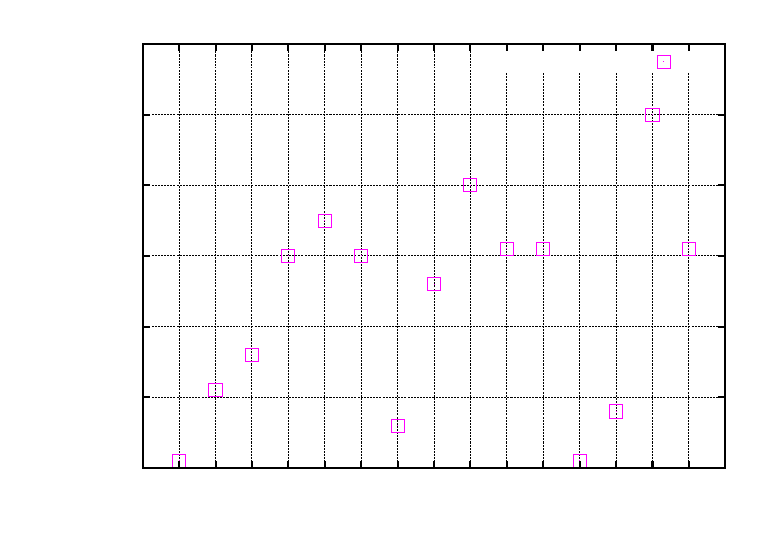
\includegraphics{../GNU/SelfTref}}%
    \gplfronttext
  \end{picture}%
\endgroup

  \caption{Selbsttest: Referenz-Spannungen}
  \label{fig:SelfTref}
\end{figure}

\begin{figure}[H]
  \begin{subfigure}[b]{9cm}
    \centering
    \resizebox{9cm}{!}{% GNUPLOT: LaTeX picture with Postscript
\begingroup
  \makeatletter
  \providecommand\color[2][]{%
    \GenericError{(gnuplot) \space\space\space\@spaces}{%
      Package color not loaded in conjunction with
      terminal option `colourtext'%
    }{See the gnuplot documentation for explanation.%
    }{Either use 'blacktext' in gnuplot or load the package
      color.sty in LaTeX.}%
    \renewcommand\color[2][]{}%
  }%
  \providecommand\includegraphics[2][]{%
    \GenericError{(gnuplot) \space\space\space\@spaces}{%
      Package graphicx or graphics not loaded%
    }{See the gnuplot documentation for explanation.%
    }{The gnuplot epslatex terminal needs graphicx.sty or graphics.sty.}%
    \renewcommand\includegraphics[2][]{}%
  }%
  \providecommand\rotatebox[2]{#2}%
  \@ifundefined{ifGPcolor}{%
    \newif\ifGPcolor
    \GPcolortrue
  }{}%
  \@ifundefined{ifGPblacktext}{%
    \newif\ifGPblacktext
    \GPblacktexttrue
  }{}%
  % define a \g@addto@macro without @ in the name:
  \let\gplgaddtomacro\g@addto@macro
  % define empty templates for all commands taking text:
  \gdef\gplbacktext{}%
  \gdef\gplfronttext{}%
  \makeatother
  \ifGPblacktext
    % no textcolor at all
    \def\colorrgb#1{}%
    \def\colorgray#1{}%
  \else
    % gray or color?
    \ifGPcolor
      \def\colorrgb#1{\color[rgb]{#1}}%
      \def\colorgray#1{\color[gray]{#1}}%
      \expandafter\def\csname LTw\endcsname{\color{white}}%
      \expandafter\def\csname LTb\endcsname{\color{black}}%
      \expandafter\def\csname LTa\endcsname{\color{black}}%
      \expandafter\def\csname LT0\endcsname{\color[rgb]{1,0,0}}%
      \expandafter\def\csname LT1\endcsname{\color[rgb]{0,1,0}}%
      \expandafter\def\csname LT2\endcsname{\color[rgb]{0,0,1}}%
      \expandafter\def\csname LT3\endcsname{\color[rgb]{1,0,1}}%
      \expandafter\def\csname LT4\endcsname{\color[rgb]{0,1,1}}%
      \expandafter\def\csname LT5\endcsname{\color[rgb]{1,1,0}}%
      \expandafter\def\csname LT6\endcsname{\color[rgb]{0,0,0}}%
      \expandafter\def\csname LT7\endcsname{\color[rgb]{1,0.3,0}}%
      \expandafter\def\csname LT8\endcsname{\color[rgb]{0.5,0.5,0.5}}%
    \else
      % gray
      \def\colorrgb#1{\color{black}}%
      \def\colorgray#1{\color[gray]{#1}}%
      \expandafter\def\csname LTw\endcsname{\color{white}}%
      \expandafter\def\csname LTb\endcsname{\color{black}}%
      \expandafter\def\csname LTa\endcsname{\color{black}}%
      \expandafter\def\csname LT0\endcsname{\color{black}}%
      \expandafter\def\csname LT1\endcsname{\color{black}}%
      \expandafter\def\csname LT2\endcsname{\color{black}}%
      \expandafter\def\csname LT3\endcsname{\color{black}}%
      \expandafter\def\csname LT4\endcsname{\color{black}}%
      \expandafter\def\csname LT5\endcsname{\color{black}}%
      \expandafter\def\csname LT6\endcsname{\color{black}}%
      \expandafter\def\csname LT7\endcsname{\color{black}}%
      \expandafter\def\csname LT8\endcsname{\color{black}}%
    \fi
  \fi
  \setlength{\unitlength}{0.0500bp}%
  \begin{picture}(7200.00,5040.00)%
    \gplgaddtomacro\gplbacktext{%
      \csname LTb\endcsname%
      \put(1078,704){\makebox(0,0)[r]{\strut{} 2480}}%
      \csname LTb\endcsname%
      \put(1078,1518){\makebox(0,0)[r]{\strut{} 2485}}%
      \csname LTb\endcsname%
      \put(1078,2332){\makebox(0,0)[r]{\strut{} 2490}}%
      \csname LTb\endcsname%
      \put(1078,3147){\makebox(0,0)[r]{\strut{} 2495}}%
      \csname LTb\endcsname%
      \put(1078,3961){\makebox(0,0)[r]{\strut{} 2500}}%
      \csname LTb\endcsname%
      \put(1078,4775){\makebox(0,0)[r]{\strut{} 2505}}%
      \csname LTb\endcsname%
      \put(1210,484){\makebox(0,0){\strut{} 0}}%
      \csname LTb\endcsname%
      \put(1560,484){\makebox(0,0){\strut{} 1}}%
      \csname LTb\endcsname%
      \put(1909,484){\makebox(0,0){\strut{} 2}}%
      \csname LTb\endcsname%
      \put(2259,484){\makebox(0,0){\strut{} 3}}%
      \csname LTb\endcsname%
      \put(2608,484){\makebox(0,0){\strut{} 4}}%
      \csname LTb\endcsname%
      \put(2958,484){\makebox(0,0){\strut{} 5}}%
      \csname LTb\endcsname%
      \put(3307,484){\makebox(0,0){\strut{} 6}}%
      \csname LTb\endcsname%
      \put(3657,484){\makebox(0,0){\strut{} 7}}%
      \csname LTb\endcsname%
      \put(4007,484){\makebox(0,0){\strut{} 8}}%
      \csname LTb\endcsname%
      \put(4356,484){\makebox(0,0){\strut{} 9}}%
      \csname LTb\endcsname%
      \put(4706,484){\makebox(0,0){\strut{} 10}}%
      \csname LTb\endcsname%
      \put(5055,484){\makebox(0,0){\strut{} 11}}%
      \csname LTb\endcsname%
      \put(5405,484){\makebox(0,0){\strut{} 12}}%
      \csname LTb\endcsname%
      \put(5754,484){\makebox(0,0){\strut{} 13}}%
      \csname LTb\endcsname%
      \put(6104,484){\makebox(0,0){\strut{} 14}}%
      \csname LTb\endcsname%
      \put(6453,484){\makebox(0,0){\strut{} 15}}%
      \csname LTb\endcsname%
      \put(6803,484){\makebox(0,0){\strut{} 16}}%
      \put(176,2739){\rotatebox{-270}{\makebox(0,0){\strut{}voltage / mV}}}%
      \put(4006,154){\makebox(0,0){\strut{}Processor number}}%
      \put(4006,4665){\makebox(0,0){\strut{}}}%
    }%
    \gplgaddtomacro\gplfronttext{%
      \csname LTb\endcsname%
      \put(5753,4602){\makebox(0,0)[r]{\strut{}RLmiddle12}}%
      \csname LTb\endcsname%
      \put(5753,4382){\makebox(0,0)[r]{\strut{}RLmiddle13}}%
      \csname LTb\endcsname%
      \put(5753,4162){\makebox(0,0)[r]{\strut{}RLmiddle23}}%
    }%
    \gplbacktext
    \put(0,0){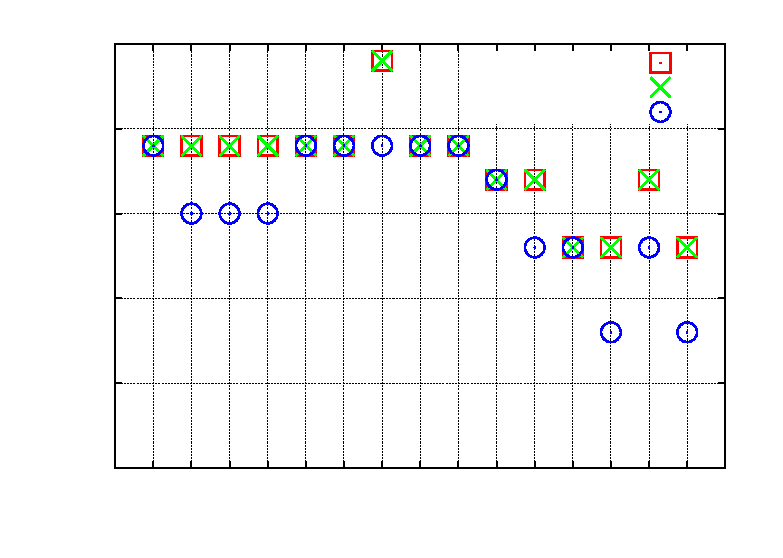
\includegraphics{../GNU/SelfTMitL}}%
    \gplfronttext
  \end{picture}%
\endgroup
}
    \caption{mit \(680 \Omega\)}
    \label{fig:SelfTMitL}
  \end{subfigure}
  ~
  \begin{subfigure}[b]{9cm}
    \centering
    \resizebox{9cm}{!}{% GNUPLOT: LaTeX picture with Postscript
\begingroup
  \makeatletter
  \providecommand\color[2][]{%
    \GenericError{(gnuplot) \space\space\space\@spaces}{%
      Package color not loaded in conjunction with
      terminal option `colourtext'%
    }{See the gnuplot documentation for explanation.%
    }{Either use 'blacktext' in gnuplot or load the package
      color.sty in LaTeX.}%
    \renewcommand\color[2][]{}%
  }%
  \providecommand\includegraphics[2][]{%
    \GenericError{(gnuplot) \space\space\space\@spaces}{%
      Package graphicx or graphics not loaded%
    }{See the gnuplot documentation for explanation.%
    }{The gnuplot epslatex terminal needs graphicx.sty or graphics.sty.}%
    \renewcommand\includegraphics[2][]{}%
  }%
  \providecommand\rotatebox[2]{#2}%
  \@ifundefined{ifGPcolor}{%
    \newif\ifGPcolor
    \GPcolortrue
  }{}%
  \@ifundefined{ifGPblacktext}{%
    \newif\ifGPblacktext
    \GPblacktexttrue
  }{}%
  % define a \g@addto@macro without @ in the name:
  \let\gplgaddtomacro\g@addto@macro
  % define empty templates for all commands taking text:
  \gdef\gplbacktext{}%
  \gdef\gplfronttext{}%
  \makeatother
  \ifGPblacktext
    % no textcolor at all
    \def\colorrgb#1{}%
    \def\colorgray#1{}%
  \else
    % gray or color?
    \ifGPcolor
      \def\colorrgb#1{\color[rgb]{#1}}%
      \def\colorgray#1{\color[gray]{#1}}%
      \expandafter\def\csname LTw\endcsname{\color{white}}%
      \expandafter\def\csname LTb\endcsname{\color{black}}%
      \expandafter\def\csname LTa\endcsname{\color{black}}%
      \expandafter\def\csname LT0\endcsname{\color[rgb]{1,0,0}}%
      \expandafter\def\csname LT1\endcsname{\color[rgb]{0,1,0}}%
      \expandafter\def\csname LT2\endcsname{\color[rgb]{0,0,1}}%
      \expandafter\def\csname LT3\endcsname{\color[rgb]{1,0,1}}%
      \expandafter\def\csname LT4\endcsname{\color[rgb]{0,1,1}}%
      \expandafter\def\csname LT5\endcsname{\color[rgb]{1,1,0}}%
      \expandafter\def\csname LT6\endcsname{\color[rgb]{0,0,0}}%
      \expandafter\def\csname LT7\endcsname{\color[rgb]{1,0.3,0}}%
      \expandafter\def\csname LT8\endcsname{\color[rgb]{0.5,0.5,0.5}}%
    \else
      % gray
      \def\colorrgb#1{\color{black}}%
      \def\colorgray#1{\color[gray]{#1}}%
      \expandafter\def\csname LTw\endcsname{\color{white}}%
      \expandafter\def\csname LTb\endcsname{\color{black}}%
      \expandafter\def\csname LTa\endcsname{\color{black}}%
      \expandafter\def\csname LT0\endcsname{\color{black}}%
      \expandafter\def\csname LT1\endcsname{\color{black}}%
      \expandafter\def\csname LT2\endcsname{\color{black}}%
      \expandafter\def\csname LT3\endcsname{\color{black}}%
      \expandafter\def\csname LT4\endcsname{\color{black}}%
      \expandafter\def\csname LT5\endcsname{\color{black}}%
      \expandafter\def\csname LT6\endcsname{\color{black}}%
      \expandafter\def\csname LT7\endcsname{\color{black}}%
      \expandafter\def\csname LT8\endcsname{\color{black}}%
    \fi
  \fi
  \setlength{\unitlength}{0.0500bp}%
  \begin{picture}(7200.00,5040.00)%
    \gplgaddtomacro\gplbacktext{%
      \csname LTb\endcsname%
      \put(1078,704){\makebox(0,0)[r]{\strut{} 2480}}%
      \csname LTb\endcsname%
      \put(1078,1518){\makebox(0,0)[r]{\strut{} 2485}}%
      \csname LTb\endcsname%
      \put(1078,2332){\makebox(0,0)[r]{\strut{} 2490}}%
      \csname LTb\endcsname%
      \put(1078,3147){\makebox(0,0)[r]{\strut{} 2495}}%
      \csname LTb\endcsname%
      \put(1078,3961){\makebox(0,0)[r]{\strut{} 2500}}%
      \csname LTb\endcsname%
      \put(1078,4775){\makebox(0,0)[r]{\strut{} 2505}}%
      \csname LTb\endcsname%
      \put(1210,484){\makebox(0,0){\strut{} 0}}%
      \csname LTb\endcsname%
      \put(1560,484){\makebox(0,0){\strut{} 1}}%
      \csname LTb\endcsname%
      \put(1909,484){\makebox(0,0){\strut{} 2}}%
      \csname LTb\endcsname%
      \put(2259,484){\makebox(0,0){\strut{} 3}}%
      \csname LTb\endcsname%
      \put(2608,484){\makebox(0,0){\strut{} 4}}%
      \csname LTb\endcsname%
      \put(2958,484){\makebox(0,0){\strut{} 5}}%
      \csname LTb\endcsname%
      \put(3307,484){\makebox(0,0){\strut{} 6}}%
      \csname LTb\endcsname%
      \put(3657,484){\makebox(0,0){\strut{} 7}}%
      \csname LTb\endcsname%
      \put(4007,484){\makebox(0,0){\strut{} 8}}%
      \csname LTb\endcsname%
      \put(4356,484){\makebox(0,0){\strut{} 9}}%
      \csname LTb\endcsname%
      \put(4706,484){\makebox(0,0){\strut{} 10}}%
      \csname LTb\endcsname%
      \put(5055,484){\makebox(0,0){\strut{} 11}}%
      \csname LTb\endcsname%
      \put(5405,484){\makebox(0,0){\strut{} 12}}%
      \csname LTb\endcsname%
      \put(5754,484){\makebox(0,0){\strut{} 13}}%
      \csname LTb\endcsname%
      \put(6104,484){\makebox(0,0){\strut{} 14}}%
      \csname LTb\endcsname%
      \put(6453,484){\makebox(0,0){\strut{} 15}}%
      \csname LTb\endcsname%
      \put(6803,484){\makebox(0,0){\strut{} 16}}%
      \put(176,2739){\rotatebox{-270}{\makebox(0,0){\strut{}voltage / mV}}}%
      \put(4006,154){\makebox(0,0){\strut{}Processor number}}%
      \put(4006,4665){\makebox(0,0){\strut{}}}%
    }%
    \gplgaddtomacro\gplfronttext{%
      \csname LTb\endcsname%
      \put(5753,4602){\makebox(0,0)[r]{\strut{}RHmiddle12}}%
      \csname LTb\endcsname%
      \put(5753,4382){\makebox(0,0)[r]{\strut{}RHmiddle13}}%
      \csname LTb\endcsname%
      \put(5753,4162){\makebox(0,0)[r]{\strut{}RHmiddle23}}%
    }%
    \gplbacktext
    \put(0,0){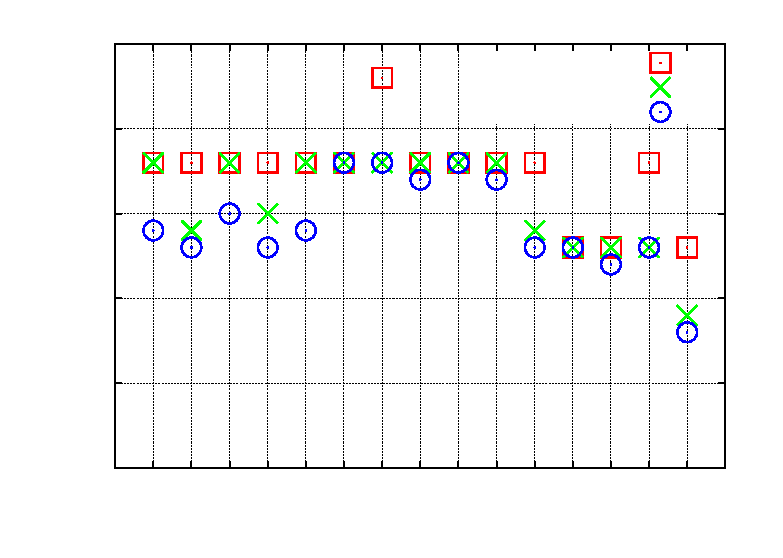
\includegraphics{../GNU/SelfTMitH}}%
    \gplfronttext
  \end{picture}%
\endgroup
}
    \caption{mit \(470 k\Omega\)}
    \label{fig:SelfTMitH}
  \end{subfigure}
  \caption{Selbsttest: Abweichung der Mittenspannung}
\end{figure}

\begin{figure}[H]
  \begin{subfigure}[b]{9cm}
  \centering
    \resizebox{9cm}{!}{% GNUPLOT: LaTeX picture with Postscript
\begingroup
  \makeatletter
  \providecommand\color[2][]{%
    \GenericError{(gnuplot) \space\space\space\@spaces}{%
      Package color not loaded in conjunction with
      terminal option `colourtext'%
    }{See the gnuplot documentation for explanation.%
    }{Either use 'blacktext' in gnuplot or load the package
      color.sty in LaTeX.}%
    \renewcommand\color[2][]{}%
  }%
  \providecommand\includegraphics[2][]{%
    \GenericError{(gnuplot) \space\space\space\@spaces}{%
      Package graphicx or graphics not loaded%
    }{See the gnuplot documentation for explanation.%
    }{The gnuplot epslatex terminal needs graphicx.sty or graphics.sty.}%
    \renewcommand\includegraphics[2][]{}%
  }%
  \providecommand\rotatebox[2]{#2}%
  \@ifundefined{ifGPcolor}{%
    \newif\ifGPcolor
    \GPcolortrue
  }{}%
  \@ifundefined{ifGPblacktext}{%
    \newif\ifGPblacktext
    \GPblacktexttrue
  }{}%
  % define a \g@addto@macro without @ in the name:
  \let\gplgaddtomacro\g@addto@macro
  % define empty templates for all commands taking text:
  \gdef\gplbacktext{}%
  \gdef\gplfronttext{}%
  \makeatother
  \ifGPblacktext
    % no textcolor at all
    \def\colorrgb#1{}%
    \def\colorgray#1{}%
  \else
    % gray or color?
    \ifGPcolor
      \def\colorrgb#1{\color[rgb]{#1}}%
      \def\colorgray#1{\color[gray]{#1}}%
      \expandafter\def\csname LTw\endcsname{\color{white}}%
      \expandafter\def\csname LTb\endcsname{\color{black}}%
      \expandafter\def\csname LTa\endcsname{\color{black}}%
      \expandafter\def\csname LT0\endcsname{\color[rgb]{1,0,0}}%
      \expandafter\def\csname LT1\endcsname{\color[rgb]{0,1,0}}%
      \expandafter\def\csname LT2\endcsname{\color[rgb]{0,0,1}}%
      \expandafter\def\csname LT3\endcsname{\color[rgb]{1,0,1}}%
      \expandafter\def\csname LT4\endcsname{\color[rgb]{0,1,1}}%
      \expandafter\def\csname LT5\endcsname{\color[rgb]{1,1,0}}%
      \expandafter\def\csname LT6\endcsname{\color[rgb]{0,0,0}}%
      \expandafter\def\csname LT7\endcsname{\color[rgb]{1,0.3,0}}%
      \expandafter\def\csname LT8\endcsname{\color[rgb]{0.5,0.5,0.5}}%
    \else
      % gray
      \def\colorrgb#1{\color{black}}%
      \def\colorgray#1{\color[gray]{#1}}%
      \expandafter\def\csname LTw\endcsname{\color{white}}%
      \expandafter\def\csname LTb\endcsname{\color{black}}%
      \expandafter\def\csname LTa\endcsname{\color{black}}%
      \expandafter\def\csname LT0\endcsname{\color{black}}%
      \expandafter\def\csname LT1\endcsname{\color{black}}%
      \expandafter\def\csname LT2\endcsname{\color{black}}%
      \expandafter\def\csname LT3\endcsname{\color{black}}%
      \expandafter\def\csname LT4\endcsname{\color{black}}%
      \expandafter\def\csname LT5\endcsname{\color{black}}%
      \expandafter\def\csname LT6\endcsname{\color{black}}%
      \expandafter\def\csname LT7\endcsname{\color{black}}%
      \expandafter\def\csname LT8\endcsname{\color{black}}%
    \fi
  \fi
  \setlength{\unitlength}{0.0500bp}%
  \begin{picture}(7200.00,5040.00)%
    \gplgaddtomacro\gplbacktext{%
      \csname LTb\endcsname%
      \put(682,704){\makebox(0,0)[r]{\strut{} 0}}%
      \csname LTb\endcsname%
      \put(682,1518){\makebox(0,0)[r]{\strut{} 1}}%
      \csname LTb\endcsname%
      \put(682,2332){\makebox(0,0)[r]{\strut{} 2}}%
      \csname LTb\endcsname%
      \put(682,3147){\makebox(0,0)[r]{\strut{} 3}}%
      \csname LTb\endcsname%
      \put(682,3961){\makebox(0,0)[r]{\strut{} 4}}%
      \csname LTb\endcsname%
      \put(682,4775){\makebox(0,0)[r]{\strut{} 5}}%
      \csname LTb\endcsname%
      \put(814,484){\makebox(0,0){\strut{} 0}}%
      \csname LTb\endcsname%
      \put(1188,484){\makebox(0,0){\strut{} 1}}%
      \csname LTb\endcsname%
      \put(1563,484){\makebox(0,0){\strut{} 2}}%
      \csname LTb\endcsname%
      \put(1937,484){\makebox(0,0){\strut{} 3}}%
      \csname LTb\endcsname%
      \put(2311,484){\makebox(0,0){\strut{} 4}}%
      \csname LTb\endcsname%
      \put(2686,484){\makebox(0,0){\strut{} 5}}%
      \csname LTb\endcsname%
      \put(3060,484){\makebox(0,0){\strut{} 6}}%
      \csname LTb\endcsname%
      \put(3434,484){\makebox(0,0){\strut{} 7}}%
      \csname LTb\endcsname%
      \put(3809,484){\makebox(0,0){\strut{} 8}}%
      \csname LTb\endcsname%
      \put(4183,484){\makebox(0,0){\strut{} 9}}%
      \csname LTb\endcsname%
      \put(4557,484){\makebox(0,0){\strut{} 10}}%
      \csname LTb\endcsname%
      \put(4931,484){\makebox(0,0){\strut{} 11}}%
      \csname LTb\endcsname%
      \put(5306,484){\makebox(0,0){\strut{} 12}}%
      \csname LTb\endcsname%
      \put(5680,484){\makebox(0,0){\strut{} 13}}%
      \csname LTb\endcsname%
      \put(6054,484){\makebox(0,0){\strut{} 14}}%
      \csname LTb\endcsname%
      \put(6429,484){\makebox(0,0){\strut{} 15}}%
      \csname LTb\endcsname%
      \put(6803,484){\makebox(0,0){\strut{} 16}}%
      \put(176,2739){\rotatebox{-270}{\makebox(0,0){\strut{}voltage / mV}}}%
      \put(3808,154){\makebox(0,0){\strut{}Processor number}}%
      \put(3808,4665){\makebox(0,0){\strut{}}}%
    }%
    \gplgaddtomacro\gplfronttext{%
      \csname LTb\endcsname%
      \put(5690,4594){\makebox(0,0)[r]{\strut{}RHbottom1}}%
      \csname LTb\endcsname%
      \put(5690,4358){\makebox(0,0)[r]{\strut{}RHbottom2}}%
      \csname LTb\endcsname%
      \put(5690,4122){\makebox(0,0)[r]{\strut{}RHbottom3}}%
    }%
    \gplbacktext
    \put(0,0){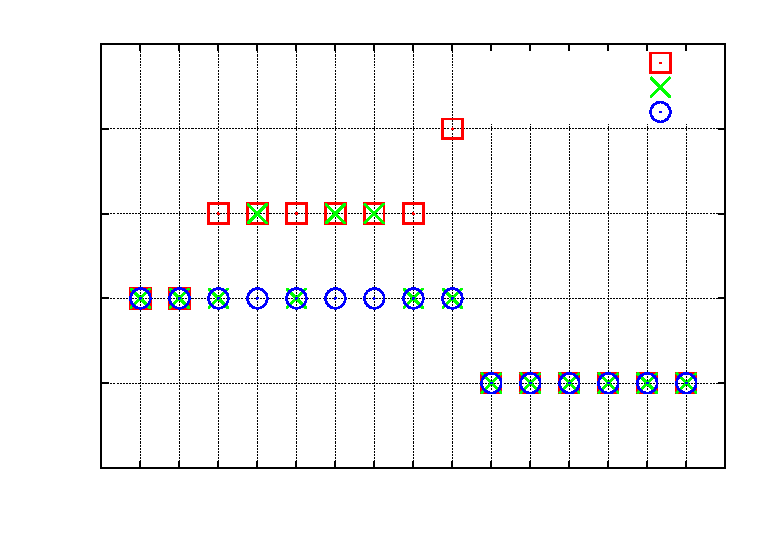
\includegraphics{../GNU/SelfTbottomH}}%
    \gplfronttext
  \end{picture}%
\endgroup
}
    \caption{mit \(470 k\Omega\) auf 0V}
    \label{fig:SelfTlowH}
  \end{subfigure}
  ~
  \begin{subfigure}[b]{9cm}
  \centering
    \resizebox{9cm}{!}{% GNUPLOT: LaTeX picture with Postscript
\begingroup
  \makeatletter
  \providecommand\color[2][]{%
    \GenericError{(gnuplot) \space\space\space\@spaces}{%
      Package color not loaded in conjunction with
      terminal option `colourtext'%
    }{See the gnuplot documentation for explanation.%
    }{Either use 'blacktext' in gnuplot or load the package
      color.sty in LaTeX.}%
    \renewcommand\color[2][]{}%
  }%
  \providecommand\includegraphics[2][]{%
    \GenericError{(gnuplot) \space\space\space\@spaces}{%
      Package graphicx or graphics not loaded%
    }{See the gnuplot documentation for explanation.%
    }{The gnuplot epslatex terminal needs graphicx.sty or graphics.sty.}%
    \renewcommand\includegraphics[2][]{}%
  }%
  \providecommand\rotatebox[2]{#2}%
  \@ifundefined{ifGPcolor}{%
    \newif\ifGPcolor
    \GPcolortrue
  }{}%
  \@ifundefined{ifGPblacktext}{%
    \newif\ifGPblacktext
    \GPblacktexttrue
  }{}%
  % define a \g@addto@macro without @ in the name:
  \let\gplgaddtomacro\g@addto@macro
  % define empty templates for all commands taking text:
  \gdef\gplbacktext{}%
  \gdef\gplfronttext{}%
  \makeatother
  \ifGPblacktext
    % no textcolor at all
    \def\colorrgb#1{}%
    \def\colorgray#1{}%
  \else
    % gray or color?
    \ifGPcolor
      \def\colorrgb#1{\color[rgb]{#1}}%
      \def\colorgray#1{\color[gray]{#1}}%
      \expandafter\def\csname LTw\endcsname{\color{white}}%
      \expandafter\def\csname LTb\endcsname{\color{black}}%
      \expandafter\def\csname LTa\endcsname{\color{black}}%
      \expandafter\def\csname LT0\endcsname{\color[rgb]{1,0,0}}%
      \expandafter\def\csname LT1\endcsname{\color[rgb]{0,1,0}}%
      \expandafter\def\csname LT2\endcsname{\color[rgb]{0,0,1}}%
      \expandafter\def\csname LT3\endcsname{\color[rgb]{1,0,1}}%
      \expandafter\def\csname LT4\endcsname{\color[rgb]{0,1,1}}%
      \expandafter\def\csname LT5\endcsname{\color[rgb]{1,1,0}}%
      \expandafter\def\csname LT6\endcsname{\color[rgb]{0,0,0}}%
      \expandafter\def\csname LT7\endcsname{\color[rgb]{1,0.3,0}}%
      \expandafter\def\csname LT8\endcsname{\color[rgb]{0.5,0.5,0.5}}%
    \else
      % gray
      \def\colorrgb#1{\color{black}}%
      \def\colorgray#1{\color[gray]{#1}}%
      \expandafter\def\csname LTw\endcsname{\color{white}}%
      \expandafter\def\csname LTb\endcsname{\color{black}}%
      \expandafter\def\csname LTa\endcsname{\color{black}}%
      \expandafter\def\csname LT0\endcsname{\color{black}}%
      \expandafter\def\csname LT1\endcsname{\color{black}}%
      \expandafter\def\csname LT2\endcsname{\color{black}}%
      \expandafter\def\csname LT3\endcsname{\color{black}}%
      \expandafter\def\csname LT4\endcsname{\color{black}}%
      \expandafter\def\csname LT5\endcsname{\color{black}}%
      \expandafter\def\csname LT6\endcsname{\color{black}}%
      \expandafter\def\csname LT7\endcsname{\color{black}}%
      \expandafter\def\csname LT8\endcsname{\color{black}}%
    \fi
  \fi
  \setlength{\unitlength}{0.0500bp}%
  \begin{picture}(7200.00,5040.00)%
    \gplgaddtomacro\gplbacktext{%
      \csname LTb\endcsname%
      \put(1078,704){\makebox(0,0)[r]{\strut{} 4996}}%
      \csname LTb\endcsname%
      \put(1078,1518){\makebox(0,0)[r]{\strut{} 4997}}%
      \csname LTb\endcsname%
      \put(1078,2332){\makebox(0,0)[r]{\strut{} 4998}}%
      \csname LTb\endcsname%
      \put(1078,3147){\makebox(0,0)[r]{\strut{} 4999}}%
      \csname LTb\endcsname%
      \put(1078,3961){\makebox(0,0)[r]{\strut{} 5000}}%
      \csname LTb\endcsname%
      \put(1078,4775){\makebox(0,0)[r]{\strut{} 5001}}%
      \csname LTb\endcsname%
      \put(1210,484){\makebox(0,0){\strut{} 0}}%
      \csname LTb\endcsname%
      \put(1560,484){\makebox(0,0){\strut{} 1}}%
      \csname LTb\endcsname%
      \put(1909,484){\makebox(0,0){\strut{} 2}}%
      \csname LTb\endcsname%
      \put(2259,484){\makebox(0,0){\strut{} 3}}%
      \csname LTb\endcsname%
      \put(2608,484){\makebox(0,0){\strut{} 4}}%
      \csname LTb\endcsname%
      \put(2958,484){\makebox(0,0){\strut{} 5}}%
      \csname LTb\endcsname%
      \put(3307,484){\makebox(0,0){\strut{} 6}}%
      \csname LTb\endcsname%
      \put(3657,484){\makebox(0,0){\strut{} 7}}%
      \csname LTb\endcsname%
      \put(4007,484){\makebox(0,0){\strut{} 8}}%
      \csname LTb\endcsname%
      \put(4356,484){\makebox(0,0){\strut{} 9}}%
      \csname LTb\endcsname%
      \put(4706,484){\makebox(0,0){\strut{} 10}}%
      \csname LTb\endcsname%
      \put(5055,484){\makebox(0,0){\strut{} 11}}%
      \csname LTb\endcsname%
      \put(5405,484){\makebox(0,0){\strut{} 12}}%
      \csname LTb\endcsname%
      \put(5754,484){\makebox(0,0){\strut{} 13}}%
      \csname LTb\endcsname%
      \put(6104,484){\makebox(0,0){\strut{} 14}}%
      \csname LTb\endcsname%
      \put(6453,484){\makebox(0,0){\strut{} 15}}%
      \csname LTb\endcsname%
      \put(6803,484){\makebox(0,0){\strut{} 16}}%
      \put(176,2739){\rotatebox{-270}{\makebox(0,0){\strut{}voltage / mV}}}%
      \put(4006,154){\makebox(0,0){\strut{}Processor number}}%
      \put(4006,4665){\makebox(0,0){\strut{}}}%
    }%
    \gplgaddtomacro\gplfronttext{%
      \csname LTb\endcsname%
      \put(5690,4594){\makebox(0,0)[r]{\strut{}RHtop1}}%
      \csname LTb\endcsname%
      \put(5690,4358){\makebox(0,0)[r]{\strut{}RHtop2}}%
      \csname LTb\endcsname%
      \put(5690,4122){\makebox(0,0)[r]{\strut{}RHtop3}}%
    }%
    \gplbacktext
    \put(0,0){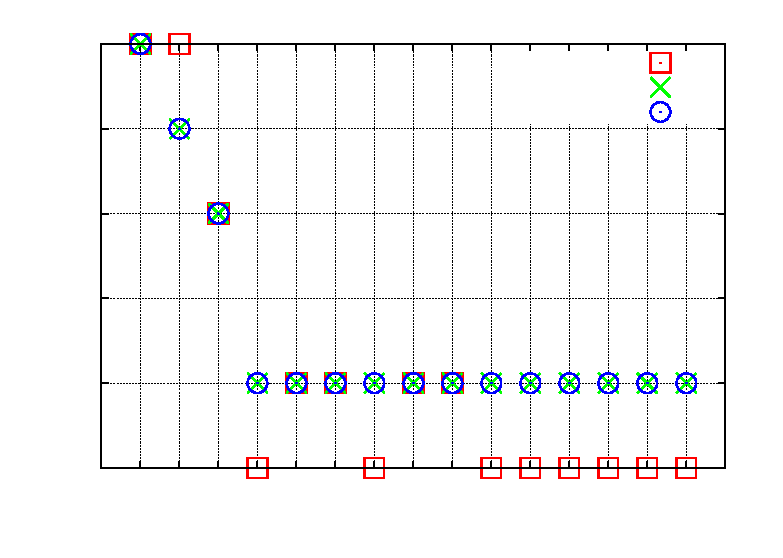
\includegraphics{../GNU/SelfTtopH}}%
    \gplfronttext
  \end{picture}%
\endgroup
}
    \caption{mit \(470 k\Omega\) auf 5V}
    \label{fig:SelfTtopH}
  \end{subfigure}
  \caption{Selbsttest: Eingangsspannung}
\end{figure}

\begin{figure}[H]
  \begin{subfigure}[b]{9cm}
  \centering
    \resizebox{9cm}{!}{% GNUPLOT: LaTeX picture with Postscript
\begingroup
  \makeatletter
  \providecommand\color[2][]{%
    \GenericError{(gnuplot) \space\space\space\@spaces}{%
      Package color not loaded in conjunction with
      terminal option `colourtext'%
    }{See the gnuplot documentation for explanation.%
    }{Either use 'blacktext' in gnuplot or load the package
      color.sty in LaTeX.}%
    \renewcommand\color[2][]{}%
  }%
  \providecommand\includegraphics[2][]{%
    \GenericError{(gnuplot) \space\space\space\@spaces}{%
      Package graphicx or graphics not loaded%
    }{See the gnuplot documentation for explanation.%
    }{The gnuplot epslatex terminal needs graphicx.sty or graphics.sty.}%
    \renewcommand\includegraphics[2][]{}%
  }%
  \providecommand\rotatebox[2]{#2}%
  \@ifundefined{ifGPcolor}{%
    \newif\ifGPcolor
    \GPcolortrue
  }{}%
  \@ifundefined{ifGPblacktext}{%
    \newif\ifGPblacktext
    \GPblacktexttrue
  }{}%
  % define a \g@addto@macro without @ in the name:
  \let\gplgaddtomacro\g@addto@macro
  % define empty templates for all commands taking text:
  \gdef\gplbacktext{}%
  \gdef\gplfronttext{}%
  \makeatother
  \ifGPblacktext
    % no textcolor at all
    \def\colorrgb#1{}%
    \def\colorgray#1{}%
  \else
    % gray or color?
    \ifGPcolor
      \def\colorrgb#1{\color[rgb]{#1}}%
      \def\colorgray#1{\color[gray]{#1}}%
      \expandafter\def\csname LTw\endcsname{\color{white}}%
      \expandafter\def\csname LTb\endcsname{\color{black}}%
      \expandafter\def\csname LTa\endcsname{\color{black}}%
      \expandafter\def\csname LT0\endcsname{\color[rgb]{1,0,0}}%
      \expandafter\def\csname LT1\endcsname{\color[rgb]{0,1,0}}%
      \expandafter\def\csname LT2\endcsname{\color[rgb]{0,0,1}}%
      \expandafter\def\csname LT3\endcsname{\color[rgb]{1,0,1}}%
      \expandafter\def\csname LT4\endcsname{\color[rgb]{0,1,1}}%
      \expandafter\def\csname LT5\endcsname{\color[rgb]{1,1,0}}%
      \expandafter\def\csname LT6\endcsname{\color[rgb]{0,0,0}}%
      \expandafter\def\csname LT7\endcsname{\color[rgb]{1,0.3,0}}%
      \expandafter\def\csname LT8\endcsname{\color[rgb]{0.5,0.5,0.5}}%
    \else
      % gray
      \def\colorrgb#1{\color{black}}%
      \def\colorgray#1{\color[gray]{#1}}%
      \expandafter\def\csname LTw\endcsname{\color{white}}%
      \expandafter\def\csname LTb\endcsname{\color{black}}%
      \expandafter\def\csname LTa\endcsname{\color{black}}%
      \expandafter\def\csname LT0\endcsname{\color{black}}%
      \expandafter\def\csname LT1\endcsname{\color{black}}%
      \expandafter\def\csname LT2\endcsname{\color{black}}%
      \expandafter\def\csname LT3\endcsname{\color{black}}%
      \expandafter\def\csname LT4\endcsname{\color{black}}%
      \expandafter\def\csname LT5\endcsname{\color{black}}%
      \expandafter\def\csname LT6\endcsname{\color{black}}%
      \expandafter\def\csname LT7\endcsname{\color{black}}%
      \expandafter\def\csname LT8\endcsname{\color{black}}%
    \fi
  \fi
  \setlength{\unitlength}{0.0500bp}%
  \begin{picture}(7200.00,5040.00)%
    \gplgaddtomacro\gplbacktext{%
      \csname LTb\endcsname%
      \put(946,704){\makebox(0,0)[r]{\strut{} 137}}%
      \csname LTb\endcsname%
      \put(946,1213){\makebox(0,0)[r]{\strut{} 138}}%
      \csname LTb\endcsname%
      \put(946,1722){\makebox(0,0)[r]{\strut{} 139}}%
      \csname LTb\endcsname%
      \put(946,2231){\makebox(0,0)[r]{\strut{} 140}}%
      \csname LTb\endcsname%
      \put(946,2740){\makebox(0,0)[r]{\strut{} 141}}%
      \csname LTb\endcsname%
      \put(946,3248){\makebox(0,0)[r]{\strut{} 142}}%
      \csname LTb\endcsname%
      \put(946,3757){\makebox(0,0)[r]{\strut{} 143}}%
      \csname LTb\endcsname%
      \put(946,4266){\makebox(0,0)[r]{\strut{} 144}}%
      \csname LTb\endcsname%
      \put(946,4775){\makebox(0,0)[r]{\strut{} 145}}%
      \csname LTb\endcsname%
      \put(1078,484){\makebox(0,0){\strut{} 0}}%
      \csname LTb\endcsname%
      \put(1436,484){\makebox(0,0){\strut{} 1}}%
      \csname LTb\endcsname%
      \put(1794,484){\makebox(0,0){\strut{} 2}}%
      \csname LTb\endcsname%
      \put(2151,484){\makebox(0,0){\strut{} 3}}%
      \csname LTb\endcsname%
      \put(2509,484){\makebox(0,0){\strut{} 4}}%
      \csname LTb\endcsname%
      \put(2867,484){\makebox(0,0){\strut{} 5}}%
      \csname LTb\endcsname%
      \put(3225,484){\makebox(0,0){\strut{} 6}}%
      \csname LTb\endcsname%
      \put(3583,484){\makebox(0,0){\strut{} 7}}%
      \csname LTb\endcsname%
      \put(3941,484){\makebox(0,0){\strut{} 8}}%
      \csname LTb\endcsname%
      \put(4298,484){\makebox(0,0){\strut{} 9}}%
      \csname LTb\endcsname%
      \put(4656,484){\makebox(0,0){\strut{} 10}}%
      \csname LTb\endcsname%
      \put(5014,484){\makebox(0,0){\strut{} 11}}%
      \csname LTb\endcsname%
      \put(5372,484){\makebox(0,0){\strut{} 12}}%
      \csname LTb\endcsname%
      \put(5730,484){\makebox(0,0){\strut{} 13}}%
      \csname LTb\endcsname%
      \put(6087,484){\makebox(0,0){\strut{} 14}}%
      \csname LTb\endcsname%
      \put(6445,484){\makebox(0,0){\strut{} 15}}%
      \csname LTb\endcsname%
      \put(6803,484){\makebox(0,0){\strut{} 16}}%
      \put(176,2739){\rotatebox{-270}{\makebox(0,0){\strut{}voltage / mV}}}%
      \put(3940,154){\makebox(0,0){\strut{}Processor number}}%
      \put(3940,4665){\makebox(0,0){\strut{}}}%
    }%
    \gplgaddtomacro\gplfronttext{%
      \csname LTb\endcsname%
      \put(5753,4602){\makebox(0,0)[r]{\strut{}RiLo1}}%
      \csname LTb\endcsname%
      \put(5753,4382){\makebox(0,0)[r]{\strut{}RiLo2}}%
      \csname LTb\endcsname%
      \put(5753,4162){\makebox(0,0)[r]{\strut{}RiLo3}}%
    }%
    \gplbacktext
    \put(0,0){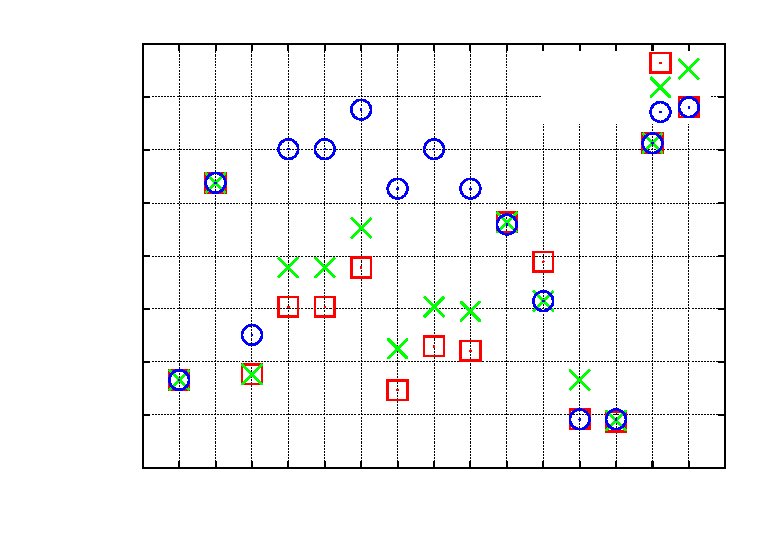
\includegraphics{../GNU/SelfTRiLo}}%
    \gplfronttext
  \end{picture}%
\endgroup
}
    \caption{mit \(680 \Omega\) auf 5V}
    \label{fig:SelfTRoL}
  \end{subfigure}
  ~
  \begin{subfigure}[b]{9cm}
  \centering
    \resizebox{9cm}{!}{% GNUPLOT: LaTeX picture with Postscript
\begingroup
  \makeatletter
  \providecommand\color[2][]{%
    \GenericError{(gnuplot) \space\space\space\@spaces}{%
      Package color not loaded in conjunction with
      terminal option `colourtext'%
    }{See the gnuplot documentation for explanation.%
    }{Either use 'blacktext' in gnuplot or load the package
      color.sty in LaTeX.}%
    \renewcommand\color[2][]{}%
  }%
  \providecommand\includegraphics[2][]{%
    \GenericError{(gnuplot) \space\space\space\@spaces}{%
      Package graphicx or graphics not loaded%
    }{See the gnuplot documentation for explanation.%
    }{The gnuplot epslatex terminal needs graphicx.sty or graphics.sty.}%
    \renewcommand\includegraphics[2][]{}%
  }%
  \providecommand\rotatebox[2]{#2}%
  \@ifundefined{ifGPcolor}{%
    \newif\ifGPcolor
    \GPcolortrue
  }{}%
  \@ifundefined{ifGPblacktext}{%
    \newif\ifGPblacktext
    \GPblacktexttrue
  }{}%
  % define a \g@addto@macro without @ in the name:
  \let\gplgaddtomacro\g@addto@macro
  % define empty templates for all commands taking text:
  \gdef\gplbacktext{}%
  \gdef\gplfronttext{}%
  \makeatother
  \ifGPblacktext
    % no textcolor at all
    \def\colorrgb#1{}%
    \def\colorgray#1{}%
  \else
    % gray or color?
    \ifGPcolor
      \def\colorrgb#1{\color[rgb]{#1}}%
      \def\colorgray#1{\color[gray]{#1}}%
      \expandafter\def\csname LTw\endcsname{\color{white}}%
      \expandafter\def\csname LTb\endcsname{\color{black}}%
      \expandafter\def\csname LTa\endcsname{\color{black}}%
      \expandafter\def\csname LT0\endcsname{\color[rgb]{1,0,0}}%
      \expandafter\def\csname LT1\endcsname{\color[rgb]{0,1,0}}%
      \expandafter\def\csname LT2\endcsname{\color[rgb]{0,0,1}}%
      \expandafter\def\csname LT3\endcsname{\color[rgb]{1,0,1}}%
      \expandafter\def\csname LT4\endcsname{\color[rgb]{0,1,1}}%
      \expandafter\def\csname LT5\endcsname{\color[rgb]{1,1,0}}%
      \expandafter\def\csname LT6\endcsname{\color[rgb]{0,0,0}}%
      \expandafter\def\csname LT7\endcsname{\color[rgb]{1,0.3,0}}%
      \expandafter\def\csname LT8\endcsname{\color[rgb]{0.5,0.5,0.5}}%
    \else
      % gray
      \def\colorrgb#1{\color{black}}%
      \def\colorgray#1{\color[gray]{#1}}%
      \expandafter\def\csname LTw\endcsname{\color{white}}%
      \expandafter\def\csname LTb\endcsname{\color{black}}%
      \expandafter\def\csname LTa\endcsname{\color{black}}%
      \expandafter\def\csname LT0\endcsname{\color{black}}%
      \expandafter\def\csname LT1\endcsname{\color{black}}%
      \expandafter\def\csname LT2\endcsname{\color{black}}%
      \expandafter\def\csname LT3\endcsname{\color{black}}%
      \expandafter\def\csname LT4\endcsname{\color{black}}%
      \expandafter\def\csname LT5\endcsname{\color{black}}%
      \expandafter\def\csname LT6\endcsname{\color{black}}%
      \expandafter\def\csname LT7\endcsname{\color{black}}%
      \expandafter\def\csname LT8\endcsname{\color{black}}%
    \fi
  \fi
  \setlength{\unitlength}{0.0500bp}%
  \begin{picture}(7200.00,5040.00)%
    \gplgaddtomacro\gplbacktext{%
      \csname LTb\endcsname%
      \put(946,704){\makebox(0,0)[r]{\strut{} 146}}%
      \csname LTb\endcsname%
      \put(946,1213){\makebox(0,0)[r]{\strut{} 148}}%
      \csname LTb\endcsname%
      \put(946,1722){\makebox(0,0)[r]{\strut{} 150}}%
      \csname LTb\endcsname%
      \put(946,2231){\makebox(0,0)[r]{\strut{} 152}}%
      \csname LTb\endcsname%
      \put(946,2740){\makebox(0,0)[r]{\strut{} 154}}%
      \csname LTb\endcsname%
      \put(946,3248){\makebox(0,0)[r]{\strut{} 156}}%
      \csname LTb\endcsname%
      \put(946,3757){\makebox(0,0)[r]{\strut{} 158}}%
      \csname LTb\endcsname%
      \put(946,4266){\makebox(0,0)[r]{\strut{} 160}}%
      \csname LTb\endcsname%
      \put(946,4775){\makebox(0,0)[r]{\strut{} 162}}%
      \csname LTb\endcsname%
      \put(1078,484){\makebox(0,0){\strut{} 0}}%
      \csname LTb\endcsname%
      \put(1436,484){\makebox(0,0){\strut{} 1}}%
      \csname LTb\endcsname%
      \put(1794,484){\makebox(0,0){\strut{} 2}}%
      \csname LTb\endcsname%
      \put(2151,484){\makebox(0,0){\strut{} 3}}%
      \csname LTb\endcsname%
      \put(2509,484){\makebox(0,0){\strut{} 4}}%
      \csname LTb\endcsname%
      \put(2867,484){\makebox(0,0){\strut{} 5}}%
      \csname LTb\endcsname%
      \put(3225,484){\makebox(0,0){\strut{} 6}}%
      \csname LTb\endcsname%
      \put(3583,484){\makebox(0,0){\strut{} 7}}%
      \csname LTb\endcsname%
      \put(3941,484){\makebox(0,0){\strut{} 8}}%
      \csname LTb\endcsname%
      \put(4298,484){\makebox(0,0){\strut{} 9}}%
      \csname LTb\endcsname%
      \put(4656,484){\makebox(0,0){\strut{} 10}}%
      \csname LTb\endcsname%
      \put(5014,484){\makebox(0,0){\strut{} 11}}%
      \csname LTb\endcsname%
      \put(5372,484){\makebox(0,0){\strut{} 12}}%
      \csname LTb\endcsname%
      \put(5730,484){\makebox(0,0){\strut{} 13}}%
      \csname LTb\endcsname%
      \put(6087,484){\makebox(0,0){\strut{} 14}}%
      \csname LTb\endcsname%
      \put(6445,484){\makebox(0,0){\strut{} 15}}%
      \csname LTb\endcsname%
      \put(6803,484){\makebox(0,0){\strut{} 16}}%
      \put(176,2739){\rotatebox{-270}{\makebox(0,0){\strut{}voltage / mV}}}%
      \put(3940,154){\makebox(0,0){\strut{}Processor number}}%
      \put(3940,4665){\makebox(0,0){\strut{}}}%
    }%
    \gplgaddtomacro\gplfronttext{%
      \csname LTb\endcsname%
      \put(5753,4602){\makebox(0,0)[r]{\strut{}RiHi1}}%
      \csname LTb\endcsname%
      \put(5753,4382){\makebox(0,0)[r]{\strut{}RiHi2}}%
      \csname LTb\endcsname%
      \put(5753,4162){\makebox(0,0)[r]{\strut{}RiHi3}}%
    }%
    \gplbacktext
    \put(0,0){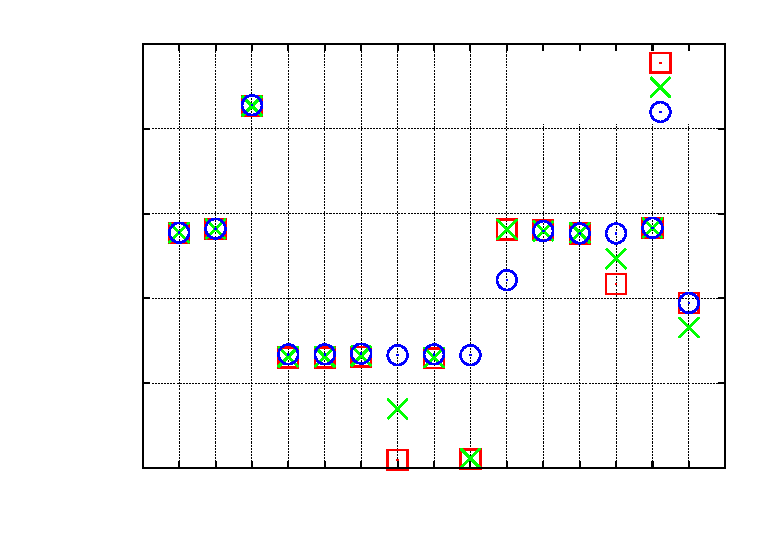
\includegraphics{../GNU/SelfTRiHi}}%
    \gplfronttext
  \end{picture}%
\endgroup
}
    \caption{mit \(680 \Omega\) auf 0V}
    \label{fig:SelfTRoH}
  \end{subfigure}
  \caption{Selbsttest: Ausgangswiderstand}
\end{figure}

\begin{figure}[H]
  \centering
  \resizebox{9cm}{!}{% GNUPLOT: LaTeX picture with Postscript
\begingroup
  \makeatletter
  \providecommand\color[2][]{%
    \GenericError{(gnuplot) \space\space\space\@spaces}{%
      Package color not loaded in conjunction with
      terminal option `colourtext'%
    }{See the gnuplot documentation for explanation.%
    }{Either use 'blacktext' in gnuplot or load the package
      color.sty in LaTeX.}%
    \renewcommand\color[2][]{}%
  }%
  \providecommand\includegraphics[2][]{%
    \GenericError{(gnuplot) \space\space\space\@spaces}{%
      Package graphicx or graphics not loaded%
    }{See the gnuplot documentation for explanation.%
    }{The gnuplot epslatex terminal needs graphicx.sty or graphics.sty.}%
    \renewcommand\includegraphics[2][]{}%
  }%
  \providecommand\rotatebox[2]{#2}%
  \@ifundefined{ifGPcolor}{%
    \newif\ifGPcolor
    \GPcolortrue
  }{}%
  \@ifundefined{ifGPblacktext}{%
    \newif\ifGPblacktext
    \GPblacktexttrue
  }{}%
  % define a \g@addto@macro without @ in the name:
  \let\gplgaddtomacro\g@addto@macro
  % define empty templates for all commands taking text:
  \gdef\gplbacktext{}%
  \gdef\gplfronttext{}%
  \makeatother
  \ifGPblacktext
    % no textcolor at all
    \def\colorrgb#1{}%
    \def\colorgray#1{}%
  \else
    % gray or color?
    \ifGPcolor
      \def\colorrgb#1{\color[rgb]{#1}}%
      \def\colorgray#1{\color[gray]{#1}}%
      \expandafter\def\csname LTw\endcsname{\color{white}}%
      \expandafter\def\csname LTb\endcsname{\color{black}}%
      \expandafter\def\csname LTa\endcsname{\color{black}}%
      \expandafter\def\csname LT0\endcsname{\color[rgb]{1,0,0}}%
      \expandafter\def\csname LT1\endcsname{\color[rgb]{0,1,0}}%
      \expandafter\def\csname LT2\endcsname{\color[rgb]{0,0,1}}%
      \expandafter\def\csname LT3\endcsname{\color[rgb]{1,0,1}}%
      \expandafter\def\csname LT4\endcsname{\color[rgb]{0,1,1}}%
      \expandafter\def\csname LT5\endcsname{\color[rgb]{1,1,0}}%
      \expandafter\def\csname LT6\endcsname{\color[rgb]{0,0,0}}%
      \expandafter\def\csname LT7\endcsname{\color[rgb]{1,0.3,0}}%
      \expandafter\def\csname LT8\endcsname{\color[rgb]{0.5,0.5,0.5}}%
    \else
      % gray
      \def\colorrgb#1{\color{black}}%
      \def\colorgray#1{\color[gray]{#1}}%
      \expandafter\def\csname LTw\endcsname{\color{white}}%
      \expandafter\def\csname LTb\endcsname{\color{black}}%
      \expandafter\def\csname LTa\endcsname{\color{black}}%
      \expandafter\def\csname LT0\endcsname{\color{black}}%
      \expandafter\def\csname LT1\endcsname{\color{black}}%
      \expandafter\def\csname LT2\endcsname{\color{black}}%
      \expandafter\def\csname LT3\endcsname{\color{black}}%
      \expandafter\def\csname LT4\endcsname{\color{black}}%
      \expandafter\def\csname LT5\endcsname{\color{black}}%
      \expandafter\def\csname LT6\endcsname{\color{black}}%
      \expandafter\def\csname LT7\endcsname{\color{black}}%
      \expandafter\def\csname LT8\endcsname{\color{black}}%
    \fi
  \fi
  \setlength{\unitlength}{0.0500bp}%
  \begin{picture}(7200.00,5040.00)%
    \gplgaddtomacro\gplbacktext{%
      \csname LTb\endcsname%
      \put(814,704){\makebox(0,0)[r]{\strut{} 36}}%
      \csname LTb\endcsname%
      \put(814,1286){\makebox(0,0)[r]{\strut{} 37}}%
      \csname LTb\endcsname%
      \put(814,1867){\makebox(0,0)[r]{\strut{} 38}}%
      \csname LTb\endcsname%
      \put(814,2449){\makebox(0,0)[r]{\strut{} 39}}%
      \csname LTb\endcsname%
      \put(814,3030){\makebox(0,0)[r]{\strut{} 40}}%
      \csname LTb\endcsname%
      \put(814,3612){\makebox(0,0)[r]{\strut{} 41}}%
      \csname LTb\endcsname%
      \put(814,4193){\makebox(0,0)[r]{\strut{} 42}}%
      \csname LTb\endcsname%
      \put(814,4775){\makebox(0,0)[r]{\strut{} 43}}%
      \csname LTb\endcsname%
      \put(946,484){\makebox(0,0){\strut{} 0}}%
      \csname LTb\endcsname%
      \put(1312,484){\makebox(0,0){\strut{} 1}}%
      \csname LTb\endcsname%
      \put(1678,484){\makebox(0,0){\strut{} 2}}%
      \csname LTb\endcsname%
      \put(2044,484){\makebox(0,0){\strut{} 3}}%
      \csname LTb\endcsname%
      \put(2410,484){\makebox(0,0){\strut{} 4}}%
      \csname LTb\endcsname%
      \put(2776,484){\makebox(0,0){\strut{} 5}}%
      \csname LTb\endcsname%
      \put(3142,484){\makebox(0,0){\strut{} 6}}%
      \csname LTb\endcsname%
      \put(3508,484){\makebox(0,0){\strut{} 7}}%
      \csname LTb\endcsname%
      \put(3875,484){\makebox(0,0){\strut{} 8}}%
      \csname LTb\endcsname%
      \put(4241,484){\makebox(0,0){\strut{} 9}}%
      \csname LTb\endcsname%
      \put(4607,484){\makebox(0,0){\strut{} 10}}%
      \csname LTb\endcsname%
      \put(4973,484){\makebox(0,0){\strut{} 11}}%
      \csname LTb\endcsname%
      \put(5339,484){\makebox(0,0){\strut{} 12}}%
      \csname LTb\endcsname%
      \put(5705,484){\makebox(0,0){\strut{} 13}}%
      \csname LTb\endcsname%
      \put(6071,484){\makebox(0,0){\strut{} 14}}%
      \csname LTb\endcsname%
      \put(6437,484){\makebox(0,0){\strut{} 15}}%
      \csname LTb\endcsname%
      \put(6803,484){\makebox(0,0){\strut{} 16}}%
      \put(176,2739){\rotatebox{-270}{\makebox(0,0){\strut{}Capacity / pF}}}%
      \put(3874,154){\makebox(0,0){\strut{}Processor number}}%
      \put(3874,4665){\makebox(0,0){\strut{}}}%
    }%
    \gplgaddtomacro\gplfronttext{%
      \csname LTb\endcsname%
      \put(5690,4594){\makebox(0,0)[r]{\strut{}CNULL1}}%
      \csname LTb\endcsname%
      \put(5690,4358){\makebox(0,0)[r]{\strut{}CNULL2}}%
      \csname LTb\endcsname%
      \put(5690,4122){\makebox(0,0)[r]{\strut{}CNULL3}}%
    }%
    \gplbacktext
    \put(0,0){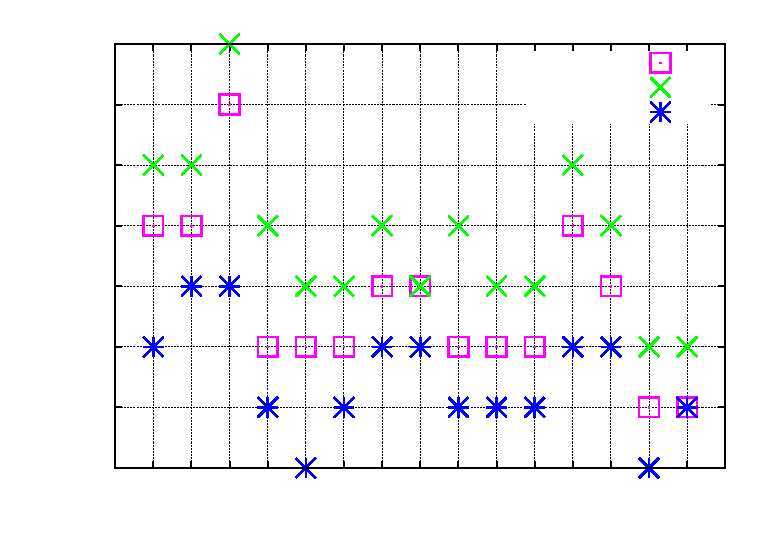
\includegraphics{../GNU/SelfTcap0}}%
    \gplfronttext
  \end{picture}%
\endgroup
}
  \caption{Selbsttest: Nullwert der Kapazit\"atsmessung}
  \label{fig:SelfTcap}
\end{figure}

\begin{figure}[H]
  \centering
  \resizebox{9cm}{!}{% GNUPLOT: LaTeX picture with Postscript
\begingroup
  \makeatletter
  \providecommand\color[2][]{%
    \GenericError{(gnuplot) \space\space\space\@spaces}{%
      Package color not loaded in conjunction with
      terminal option `colourtext'%
    }{See the gnuplot documentation for explanation.%
    }{Either use 'blacktext' in gnuplot or load the package
      color.sty in LaTeX.}%
    \renewcommand\color[2][]{}%
  }%
  \providecommand\includegraphics[2][]{%
    \GenericError{(gnuplot) \space\space\space\@spaces}{%
      Package graphicx or graphics not loaded%
    }{See the gnuplot documentation for explanation.%
    }{The gnuplot epslatex terminal needs graphicx.sty or graphics.sty.}%
    \renewcommand\includegraphics[2][]{}%
  }%
  \providecommand\rotatebox[2]{#2}%
  \@ifundefined{ifGPcolor}{%
    \newif\ifGPcolor
    \GPcolortrue
  }{}%
  \@ifundefined{ifGPblacktext}{%
    \newif\ifGPblacktext
    \GPblacktexttrue
  }{}%
  % define a \g@addto@macro without @ in the name:
  \let\gplgaddtomacro\g@addto@macro
  % define empty templates for all commands taking text:
  \gdef\gplbacktext{}%
  \gdef\gplfronttext{}%
  \makeatother
  \ifGPblacktext
    % no textcolor at all
    \def\colorrgb#1{}%
    \def\colorgray#1{}%
  \else
    % gray or color?
    \ifGPcolor
      \def\colorrgb#1{\color[rgb]{#1}}%
      \def\colorgray#1{\color[gray]{#1}}%
      \expandafter\def\csname LTw\endcsname{\color{white}}%
      \expandafter\def\csname LTb\endcsname{\color{black}}%
      \expandafter\def\csname LTa\endcsname{\color{black}}%
      \expandafter\def\csname LT0\endcsname{\color[rgb]{1,0,0}}%
      \expandafter\def\csname LT1\endcsname{\color[rgb]{0,1,0}}%
      \expandafter\def\csname LT2\endcsname{\color[rgb]{0,0,1}}%
      \expandafter\def\csname LT3\endcsname{\color[rgb]{1,0,1}}%
      \expandafter\def\csname LT4\endcsname{\color[rgb]{0,1,1}}%
      \expandafter\def\csname LT5\endcsname{\color[rgb]{1,1,0}}%
      \expandafter\def\csname LT6\endcsname{\color[rgb]{0,0,0}}%
      \expandafter\def\csname LT7\endcsname{\color[rgb]{1,0.3,0}}%
      \expandafter\def\csname LT8\endcsname{\color[rgb]{0.5,0.5,0.5}}%
    \else
      % gray
      \def\colorrgb#1{\color{black}}%
      \def\colorgray#1{\color[gray]{#1}}%
      \expandafter\def\csname LTw\endcsname{\color{white}}%
      \expandafter\def\csname LTb\endcsname{\color{black}}%
      \expandafter\def\csname LTa\endcsname{\color{black}}%
      \expandafter\def\csname LT0\endcsname{\color{black}}%
      \expandafter\def\csname LT1\endcsname{\color{black}}%
      \expandafter\def\csname LT2\endcsname{\color{black}}%
      \expandafter\def\csname LT3\endcsname{\color{black}}%
      \expandafter\def\csname LT4\endcsname{\color{black}}%
      \expandafter\def\csname LT5\endcsname{\color{black}}%
      \expandafter\def\csname LT6\endcsname{\color{black}}%
      \expandafter\def\csname LT7\endcsname{\color{black}}%
      \expandafter\def\csname LT8\endcsname{\color{black}}%
    \fi
  \fi
  \setlength{\unitlength}{0.0500bp}%
  \begin{picture}(7200.00,5040.00)%
    \gplgaddtomacro\gplbacktext{%
      \csname LTb\endcsname%
      \put(814,704){\makebox(0,0)[r]{\strut{}-60}}%
      \csname LTb\endcsname%
      \put(814,1286){\makebox(0,0)[r]{\strut{}-40}}%
      \csname LTb\endcsname%
      \put(814,1867){\makebox(0,0)[r]{\strut{}-20}}%
      \csname LTb\endcsname%
      \put(814,2449){\makebox(0,0)[r]{\strut{} 0}}%
      \csname LTb\endcsname%
      \put(814,3030){\makebox(0,0)[r]{\strut{} 20}}%
      \csname LTb\endcsname%
      \put(814,3612){\makebox(0,0)[r]{\strut{} 40}}%
      \csname LTb\endcsname%
      \put(814,4193){\makebox(0,0)[r]{\strut{} 60}}%
      \csname LTb\endcsname%
      \put(814,4775){\makebox(0,0)[r]{\strut{} 80}}%
      \csname LTb\endcsname%
      \put(946,484){\makebox(0,0){\strut{} 0}}%
      \csname LTb\endcsname%
      \put(1312,484){\makebox(0,0){\strut{} 1}}%
      \csname LTb\endcsname%
      \put(1678,484){\makebox(0,0){\strut{} 2}}%
      \csname LTb\endcsname%
      \put(2044,484){\makebox(0,0){\strut{} 3}}%
      \csname LTb\endcsname%
      \put(2410,484){\makebox(0,0){\strut{} 4}}%
      \csname LTb\endcsname%
      \put(2776,484){\makebox(0,0){\strut{} 5}}%
      \csname LTb\endcsname%
      \put(3142,484){\makebox(0,0){\strut{} 6}}%
      \csname LTb\endcsname%
      \put(3508,484){\makebox(0,0){\strut{} 7}}%
      \csname LTb\endcsname%
      \put(3875,484){\makebox(0,0){\strut{} 8}}%
      \csname LTb\endcsname%
      \put(4241,484){\makebox(0,0){\strut{} 9}}%
      \csname LTb\endcsname%
      \put(4607,484){\makebox(0,0){\strut{} 10}}%
      \csname LTb\endcsname%
      \put(4973,484){\makebox(0,0){\strut{} 11}}%
      \csname LTb\endcsname%
      \put(5339,484){\makebox(0,0){\strut{} 12}}%
      \csname LTb\endcsname%
      \put(5705,484){\makebox(0,0){\strut{} 13}}%
      \csname LTb\endcsname%
      \put(6071,484){\makebox(0,0){\strut{} 14}}%
      \csname LTb\endcsname%
      \put(6437,484){\makebox(0,0){\strut{} 15}}%
      \csname LTb\endcsname%
      \put(6803,484){\makebox(0,0){\strut{} 16}}%
      \put(176,2739){\rotatebox{-270}{\makebox(0,0){\strut{}Voltage correction / mV}}}%
      \put(3874,154){\makebox(0,0){\strut{}Processor number}}%
      \put(3874,4665){\makebox(0,0){\strut{}}}%
    }%
    \gplgaddtomacro\gplfronttext{%
      \csname LTb\endcsname%
      \put(5690,4594){\makebox(0,0)[r]{\strut{}REF\_C\_KORR}}%
      \csname LTb\endcsname%
      \put(5690,4358){\makebox(0,0)[r]{\strut{}REF\_R\_KORR}}%
    }%
    \gplbacktext
    \put(0,0){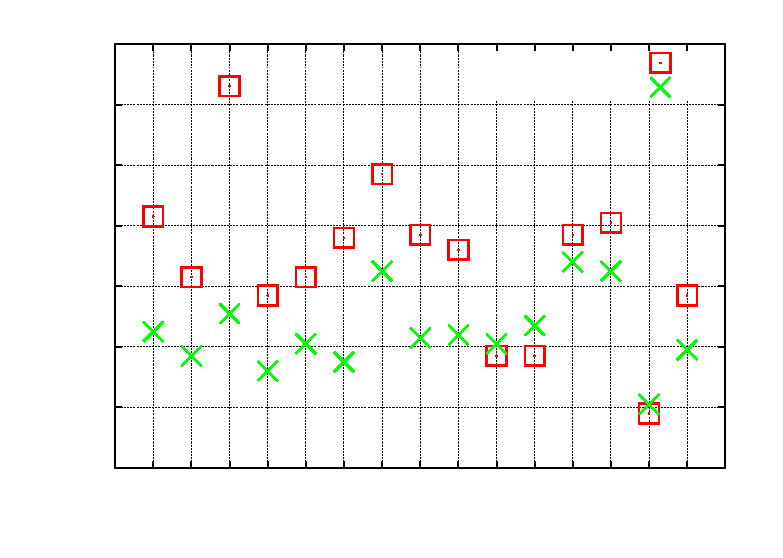
\includegraphics{../GNU/SelfTrefKorr}}%
    \gplfronttext
  \end{picture}%
\endgroup
}
  \caption{Selbsttest: Korrekturwerte nach automatischer Kalibration}
  \label{fig:SelfTrefKorr}
\end{figure}

Zuletzt m\"ochte ich die Differenzen der am AREF Pin mit einem Multimeter
gemessenen Spannungen und der intern mit dem ADC gemessenen Referenzspannungen der
15 verschiedenen ATmega Prozessoren und die mit dem automatischen Abgleich
gefundenen Korrekturspannung (REF\_R\_KORR) in Abbildung~\ref{fig:SelfTrefDiff} gegen\"uberstellen.
Sie k\"onnen sehen, da"s die Werte der automatischen Kalibration nahezu den extern
gemessenen Referenz-Spannungswerten folgen.

\begin{figure}[H]
  \centering
  \resizebox{9cm}{!}{% GNUPLOT: LaTeX picture with Postscript
\begingroup
  \makeatletter
  \providecommand\color[2][]{%
    \GenericError{(gnuplot) \space\space\space\@spaces}{%
      Package color not loaded in conjunction with
      terminal option `colourtext'%
    }{See the gnuplot documentation for explanation.%
    }{Either use 'blacktext' in gnuplot or load the package
      color.sty in LaTeX.}%
    \renewcommand\color[2][]{}%
  }%
  \providecommand\includegraphics[2][]{%
    \GenericError{(gnuplot) \space\space\space\@spaces}{%
      Package graphicx or graphics not loaded%
    }{See the gnuplot documentation for explanation.%
    }{The gnuplot epslatex terminal needs graphicx.sty or graphics.sty.}%
    \renewcommand\includegraphics[2][]{}%
  }%
  \providecommand\rotatebox[2]{#2}%
  \@ifundefined{ifGPcolor}{%
    \newif\ifGPcolor
    \GPcolortrue
  }{}%
  \@ifundefined{ifGPblacktext}{%
    \newif\ifGPblacktext
    \GPblacktexttrue
  }{}%
  % define a \g@addto@macro without @ in the name:
  \let\gplgaddtomacro\g@addto@macro
  % define empty templates for all commands taking text:
  \gdef\gplbacktext{}%
  \gdef\gplfronttext{}%
  \makeatother
  \ifGPblacktext
    % no textcolor at all
    \def\colorrgb#1{}%
    \def\colorgray#1{}%
  \else
    % gray or color?
    \ifGPcolor
      \def\colorrgb#1{\color[rgb]{#1}}%
      \def\colorgray#1{\color[gray]{#1}}%
      \expandafter\def\csname LTw\endcsname{\color{white}}%
      \expandafter\def\csname LTb\endcsname{\color{black}}%
      \expandafter\def\csname LTa\endcsname{\color{black}}%
      \expandafter\def\csname LT0\endcsname{\color[rgb]{1,0,0}}%
      \expandafter\def\csname LT1\endcsname{\color[rgb]{0,1,0}}%
      \expandafter\def\csname LT2\endcsname{\color[rgb]{0,0,1}}%
      \expandafter\def\csname LT3\endcsname{\color[rgb]{1,0,1}}%
      \expandafter\def\csname LT4\endcsname{\color[rgb]{0,1,1}}%
      \expandafter\def\csname LT5\endcsname{\color[rgb]{1,1,0}}%
      \expandafter\def\csname LT6\endcsname{\color[rgb]{0,0,0}}%
      \expandafter\def\csname LT7\endcsname{\color[rgb]{1,0.3,0}}%
      \expandafter\def\csname LT8\endcsname{\color[rgb]{0.5,0.5,0.5}}%
    \else
      % gray
      \def\colorrgb#1{\color{black}}%
      \def\colorgray#1{\color[gray]{#1}}%
      \expandafter\def\csname LTw\endcsname{\color{white}}%
      \expandafter\def\csname LTb\endcsname{\color{black}}%
      \expandafter\def\csname LTa\endcsname{\color{black}}%
      \expandafter\def\csname LT0\endcsname{\color{black}}%
      \expandafter\def\csname LT1\endcsname{\color{black}}%
      \expandafter\def\csname LT2\endcsname{\color{black}}%
      \expandafter\def\csname LT3\endcsname{\color{black}}%
      \expandafter\def\csname LT4\endcsname{\color{black}}%
      \expandafter\def\csname LT5\endcsname{\color{black}}%
      \expandafter\def\csname LT6\endcsname{\color{black}}%
      \expandafter\def\csname LT7\endcsname{\color{black}}%
      \expandafter\def\csname LT8\endcsname{\color{black}}%
    \fi
  \fi
  \setlength{\unitlength}{0.0500bp}%
  \begin{picture}(7200.00,5040.00)%
    \gplgaddtomacro\gplbacktext{%
      \csname LTb\endcsname%
      \put(814,704){\makebox(0,0)[r]{\strut{}-40}}%
      \csname LTb\endcsname%
      \put(814,1213){\makebox(0,0)[r]{\strut{}-30}}%
      \csname LTb\endcsname%
      \put(814,1722){\makebox(0,0)[r]{\strut{}-20}}%
      \csname LTb\endcsname%
      \put(814,2231){\makebox(0,0)[r]{\strut{}-10}}%
      \csname LTb\endcsname%
      \put(814,2740){\makebox(0,0)[r]{\strut{} 0}}%
      \csname LTb\endcsname%
      \put(814,3248){\makebox(0,0)[r]{\strut{} 10}}%
      \csname LTb\endcsname%
      \put(814,3757){\makebox(0,0)[r]{\strut{} 20}}%
      \csname LTb\endcsname%
      \put(814,4266){\makebox(0,0)[r]{\strut{} 30}}%
      \csname LTb\endcsname%
      \put(814,4775){\makebox(0,0)[r]{\strut{} 40}}%
      \csname LTb\endcsname%
      \put(946,484){\makebox(0,0){\strut{} 0}}%
      \csname LTb\endcsname%
      \put(1312,484){\makebox(0,0){\strut{} 1}}%
      \csname LTb\endcsname%
      \put(1678,484){\makebox(0,0){\strut{} 2}}%
      \csname LTb\endcsname%
      \put(2044,484){\makebox(0,0){\strut{} 3}}%
      \csname LTb\endcsname%
      \put(2410,484){\makebox(0,0){\strut{} 4}}%
      \csname LTb\endcsname%
      \put(2776,484){\makebox(0,0){\strut{} 5}}%
      \csname LTb\endcsname%
      \put(3142,484){\makebox(0,0){\strut{} 6}}%
      \csname LTb\endcsname%
      \put(3508,484){\makebox(0,0){\strut{} 7}}%
      \csname LTb\endcsname%
      \put(3875,484){\makebox(0,0){\strut{} 8}}%
      \csname LTb\endcsname%
      \put(4241,484){\makebox(0,0){\strut{} 9}}%
      \csname LTb\endcsname%
      \put(4607,484){\makebox(0,0){\strut{} 10}}%
      \csname LTb\endcsname%
      \put(4973,484){\makebox(0,0){\strut{} 11}}%
      \csname LTb\endcsname%
      \put(5339,484){\makebox(0,0){\strut{} 12}}%
      \csname LTb\endcsname%
      \put(5705,484){\makebox(0,0){\strut{} 13}}%
      \csname LTb\endcsname%
      \put(6071,484){\makebox(0,0){\strut{} 14}}%
      \csname LTb\endcsname%
      \put(6437,484){\makebox(0,0){\strut{} 15}}%
      \csname LTb\endcsname%
      \put(6803,484){\makebox(0,0){\strut{} 16}}%
      \put(176,2739){\rotatebox{-270}{\makebox(0,0){\strut{}Voltage difference / mV}}}%
      \put(3874,154){\makebox(0,0){\strut{}Processor number}}%
      \put(3874,4665){\makebox(0,0){\strut{}}}%
    }%
    \gplgaddtomacro\gplfronttext{%
      \csname LTb\endcsname%
      \put(5690,4594){\makebox(0,0)[r]{\strut{}AREF - REF}}%
      \csname LTb\endcsname%
      \put(5690,4358){\makebox(0,0)[r]{\strut{}REF\_R\_KORR}}%
    }%
    \gplbacktext
    \put(0,0){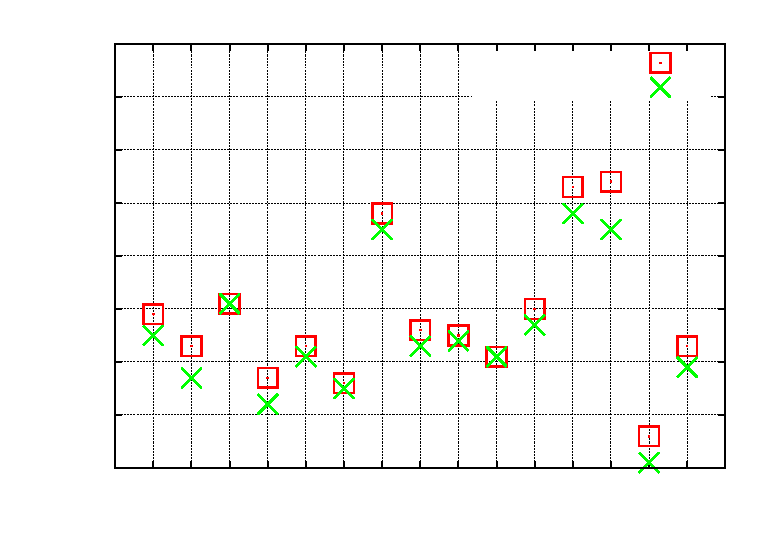
\includegraphics{../GNU/SelfTrefDiff}}%
    \gplfronttext
  \end{picture}%
\endgroup
}
  \caption{Selbsttest: Spannungsdifferenz der internen Referenz}
  \label{fig:SelfTrefDiff}
\end{figure}

